%!TEX root = draft.tex
%\newcommand{\seqPQ}{\mathsf{SeqPQ}}

\section{Compositionality of Distributed Linearizability}
\label{sec:compositionality of distributed linearizability}

\textblue{
This section should give three results of the form: if $o_1$ is linearizable w.r.t. $S_1$ and $o_2$ is linearizable w.r.t. $S_2$, and ???, then $o_1 \otimes o_2$ is linearizable w.r.t. $S_1\times S_2$ (the 2-object spec defined by interleavings). ??? may be an additional condition, while $\otimes$ is an "operator" for composing two CRDT implementations. Every result will have a different $\otimes$ operator.
\begin{itemize}
\item \gpnote*{}{Start with some counter-examples of compositionality (Check with the intro)}
\item T0 + T0: ??? = $S_1$ and $S_2$ are $T0$-specs, and $\otimes$ is the trivial composition (the "unsynchronized" product)
\item T1 + T1: ??? = $S_1$ and $S_2$ are $T1$-specs, and $\otimes$ is the "shared counter" composition (the "unsynchronized" product with a restriction on the set of generated histories)
\item T0 + T1: ??? = $S_1$ is a $T_0$ spec, and $S_2$ is a $T1$-spec, and $\otimes$ is the "global causal delivery" composition (the "unsynchronized" product with a restriction on the set of generated histories)
\end{itemize}
Also, we should prove that composing two $T0$, resp., $T1$, specs results in a $T0$, resp., $T1$ spec, and composing a $T0$ with $T1$ results in a $T1$. With this, the extension to sets of objects is straightforward:  compose all $T0$ and independently, all $T1$, then compose the two resulting objects.}

\gpnote*{}{Are there things that are neither T0 nor T1?: Not in our paper}



\subsection{T0-Linearizability and T1-Linearizability}
\label{subsec:t0-linearizability and t1-linearizability}

In this section, our goal is to give a modular verification for \crdtlin. Let us start with how to ensure the compositionality of a history. A history $\ahis$ is compositional, if when we prove that for each object $\aobj$, $\ahis \uparrow_{\aobj}$ is \crdtlinearizable{} w.r.t the corresponding specification $\Spec$, then, we obtain that $\ahis$ is \crdtlinearizable{}.


In \figurename~\ref{fig:an example of linearization of single objects do not imply a linearization of the whole history} we show an example when \crdtlinearization{} of single objects can not be used to construct the \crdtlinearization{} of the whole history. The history $\ahis$ of \figurename~\ref{fig:an example of linearization of single objects do not imply a linearization of the whole history} contains operations of two or-set objects $\aobj_1$ and $\aobj_2$. To distinguish them, the operations of $\aobj_1$ is drew with unfilled circle while the operations of $\aobj_2$ is drew with filled circle, and we list the object of each operation. We can see that $\mathit{add}(a) \cdot \mathit{add}(b)$ and $\mathit{add}(c) \cdot \mathit{add}(d)$ are \crdtlinearization{} for $\ahis \uparrow_{\aobj_1}$ and $\ahis \uparrow_{\aobj_2}$, respectively. However, since composing these two \crdtlinearization{} brings a cycle, there can not be any \crdtlinearization{} of $\ahis$ consistent with these two \crdtlinearization{} of $\ahis \uparrow_{\aobj_1}$ and $\ahis \uparrow_{\aobj_2}$.

\begin{figure}[t]
  \centering
  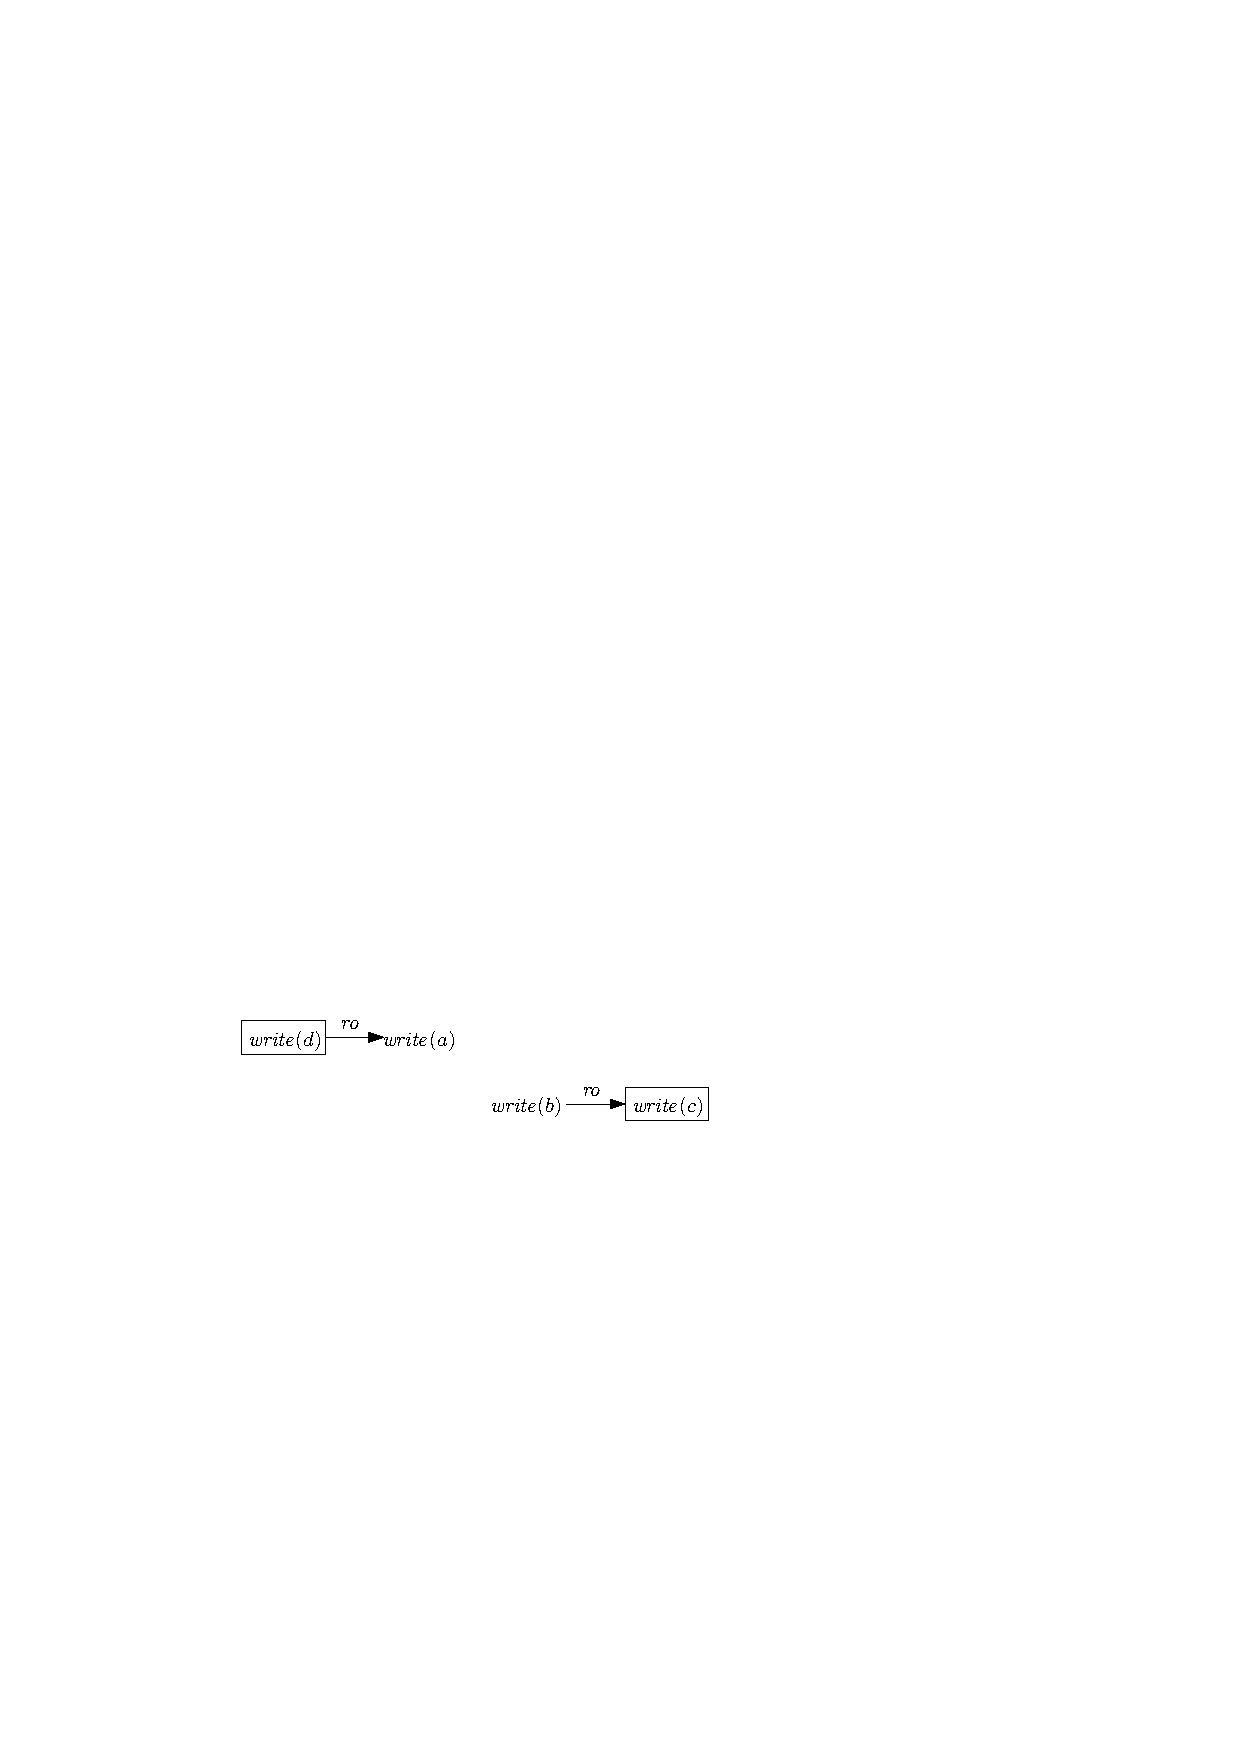
\includegraphics[width=0.35 \textwidth]{figures/TwoSubLin-NotaGlobalLin.pdf}
\vspace{-10pt}
  \caption{An example where \crdtlinearization{} of single objects, $\mathit{add}(a) \cdot \mathit{add}(b)$ and $\mathit{add}(c) \cdot \mathit{add}(d)$, can not be used to generate \crdtlinearization{} of the whole history.}
  \label{fig:an example of linearization of single objects do not imply a linearization of the whole history}
\end{figure}

A order $R$ is a interval-order, if $(\aop_1,\aop_2), (\aop_3,\aop_4) \in R$ implies that $(o_1,o_4) \in R \vee (o_3,o_2) \in R$. There is a difference between \crdtlin{} and the linearizability of \cite{HerlihyW90}: the visibility relation of \crdtlin{} is not a interval-order, while the happen-before relation in \cite{HerlihyW90} is a interval-order. The compositionality proof of \cite{HerlihyW90} proves that we can compose linearization of projection of each object into a linearization of the whole history, and such proof relies on the property of interval-order.

Although we can not directly compose smaller \crdtlinearization{} into a bigger \crdtlinearization{} directly, we can do this work by using some permutations of smaller \crdtlinearization{}. For example, for the history $\ahis$ of \figurename~\ref{fig:an example of linearization of single objects do not imply a linearization of the whole history}, we can see that $\mathit{write}(d) \cdot \mathit{write}(c)$, a permutation of \crdtlinearization{} $\mathit{write}(c) \cdot \mathit{write}(d)$ that preserves visibility relation, is also a \crdtlinearization{} of operations of $\aobj_2$, and $\ahis$ has a \crdtlinearization{} $\mathit{write}(d) \cdot \mathit{write}(a) \cdot \mathit{write}(b) \cdot \mathit{write}(c)$, which is consistent with both $\mathit{write}(a) \cdot \mathit{write}(b)$ and $\mathit{write}(d) \cdot \mathit{write}(c)$. Based on above intuition, we propose \tzerolin{} and \tonelin{}. Both of them are sub-class of \crdtlin{} and require that certain permutation of a \crdtlinearization{} is still a \crdtlinearization{}.

\begin{definition}[\tzerolin{}]
\label{definition:t0-linearizability}
A single-object history $\ahis$ is \tzerolinearizable{} w.r.t a sequential specification \Spec{}, if $\ahis$ is \crdtlinearizable{} w.r.t \Spec{}, and each specification sequence $(\alabelset, \aseqord)$ consistent with visibility order is a \crdtlinearization{}.
\end{definition}

We say a specification sequence $(\alabelset, \aseqord)$ be consistent with timestamp order, if the time-stamp of operation $\aobj_1$ being less than the timestamp of $\aobj_2$ implies that $\aobj_1$ being before $\aobj_2$ in $\aseqord$, and if $(\aobj_3,\aobj_4) \in \avisord$, then the timestamp of $\aobj_3$ is less or equal to the timestamp of $\aobj_4$.

\begin{definition}[\tonelin{}]
\label{definition:t1-linearizability}
A single-object history $\ahis$ is \tonelinearizable{} w.r.t a sequential specification \Spec{}, if $\ahis$ is \crdtlinearizable{} w.r.t \Spec{}, and each specification sequence $(\alabelset, \aseqord)$ consistent with visibility order and timestamp order is a \crdtlinearization{}.
\end{definition}






\subsection{Composing Histories}
\label{lemma:composing histories}

In this subsection, we consider the case when we are given a history $\ahis$ where $\ahis \uparrow_{\aobj}$ is \crdtlinearizable{} w.r.t its corresponding sequential specification $\Spec{}$ for each object $\aobj$, then what is the condition needed to ensure $\ahis$ being \crdtlinearizable.

The following lemma states that, if each object is \tzerolinearizable{}, then the whole history is \crdtlinearizable{}. Its proof can be found in Appendix \ref{subsec:appendix proofs of lemma several t0-specifications can be composed}.

\begin{restatable}{lemma}{composingTZero}
\label{lemma:several t0-specifications can be composed}
Given a multi-object history $\ahis$. If for each of its object $\aobj$, $\ahis \uparrow_{\aobj}$ is \tzerolinearizable{}, then, $\ahis$ is \crdtlinearizable{}.
\end{restatable}

\begin {proof} (Sketch):

We construct a \crdtlinearization $(\alabelset, \aseqord)$ of $h$ step by step by always choosing an operation that is minimal w.r.t $\avisord$. Since the visibility relation is acyclic, finally all operations of $\ahis$ will be put in $\alabelset$. Since each object use \tzerolin{} and $\aseqord$ is obviously consistent with the visibility relation, we can see that $(\alabelset, \aseqord)$ is a \crdtlinearization of $\ahis$. $\qed$
\end {proof}


However, %if each object is either \tzerolinearizable{} or \tonelinearizable{}, and
when at least one object is \tonelinearizable{} w.r.t its corresponding sequential specification, then it is possible that the whole history is not \crdtlinearizable. In \figurename~\ref{fig:a failed example of composing a multi-value register with a last-write-win register} we show an example when there is one \tonelinearizable{} object and one \tzerolinearizable{} object. The history $\ahis$ of \figurename~\ref{fig:a failed example of composing a multi-value register with a last-write-win register} contains operations of a or-set object $\aobj_1$ and a list object $\aobj_2$. Here we assume that $\ats_1 < \ats_2$. We can see that $h \uparrow_{\aobj_1}$ and $h \uparrow_{\aobj_2}$ are \crdtlinearizable, and the only possible linearization of $h \uparrow_{\aobj_1}$ and $h \uparrow_{\aobj_2}$ is $\mathit{write}(a) \cdot \mathit{write}(b)$ and $\mathit{write}(c,\circ) \cdot \mathit{write}(d,\circ) \cdot \mathit{read}() \Rightarrow d \cdot c$, respectively. However, the whole history $\ahis$ is not \crdtlinearizable, since there is a cycle in smaller linearizations.

\begin{figure}[t]
  \centering
  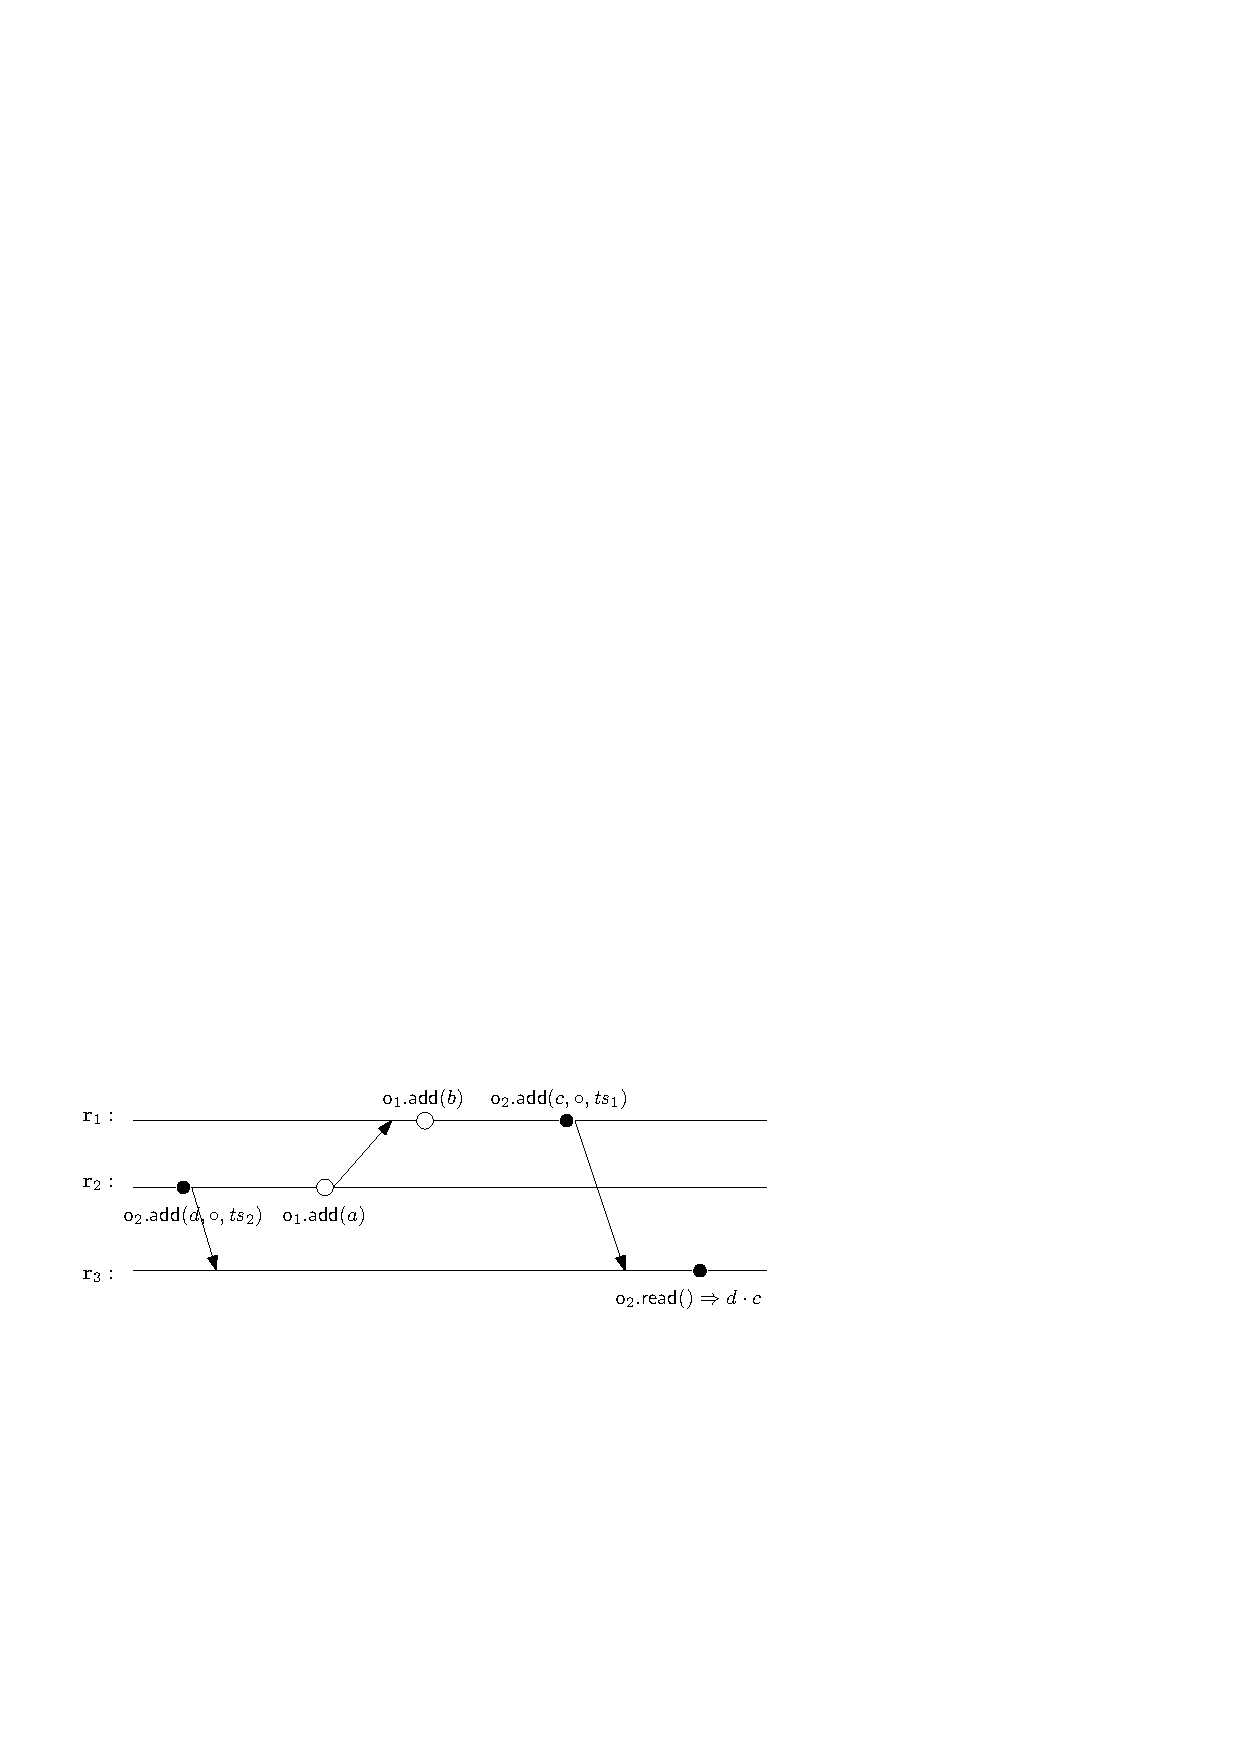
\includegraphics[width=0.6 \textwidth]{figures/MVReg-LWWReg-Nocd.pdf}
\vspace{-10pt}
  \caption{A failed example of composing a \tzerolinearizable or-set object $\aobj_1$ and a \tonelinearizable list object $\aobj_2$, where $\mathit{ts}_1 < \mathit{ts}_2$.}
  \label{fig:a failed example of composing a multi-value register with a last-write-win register}
\end{figure}

To get rid of such problem, we additionally require the visibility relation to be transitive. The following lemma states that, if there is only one object being \tonelinearizable{}, then transitive visibility relation ensures the whole history to be \crdtlinearizable{}. Its proof can be found in Appendix \ref{subsec:appendix proofs of lemma several t0-specifications and one t1-specification can be composed}.

\begin{restatable}{lemma}{composingTZeroAndOneTOne}
\label{lemma:several t0-specifications and one t1-specification can be composed}
Given a multi-object history $\ahis$ with transitive visibility relation. If for one object $\aobj$, $\ahis \uparrow_{\aobj}$ is \tonelinearizable{}, and for other object $\aobj'$, $\ahis \uparrow_{\aobj'}$ is \tzerolinearizable{}, then, $\ahis$ is \crdtlinearizable{}.
\end{restatable}

\begin {proof} (Sketch):

We construct a \crdtlinearization $(\alabelset, \aseqord)$ of $h$ step by step by always choosing either an operation of $\aobj'$ that is minimal w.r.t $\avisord$, or an operation of $\aobj$ that is minimal w.r.t $\avisord$ and timestamp order. Once such process terminates with all operations of $\ahis$ put in $\alabelset$, since $\aseqord$ is obviously consistent with the visibility relation, and $\aseqord \uparrow_{\aobj}$ is obviously consistent with the timestamp order, we know that $(\alabelset, \aseqord)$ is a \crdtlinearization of $\ahis$.

We proce that such process terminates with all operations of $\ahis$ put in $\alabelset$ by contradiction. Assume such process terminates while a set $S$ of operations is not put into $\alabelset$ yet. It is easy to see that $S$ contains only operation of $\aobj$. Let $\alabel$ be the operation of $S$ with minimal timestamp, then it is easy to see that $\alabel$ is not minimal w.r.t $\avisord$ in $S$. There exists operations $\alabel_1,\ldots,\alabel_k \in S$, such that $\alabel$ is minimal w.r.t $\avisord$ in $S$ but not minimal w.r.t timestamp order, and $(\alabel_1,\alabel_2),\ldots,(\alabel_k,\alabel) \in \avisord$. Since the visibility is transitive, we have that $(\alabel_1,\alabel) \in \avisord$ while the timestamp of $\alabel_1$ is larger than the timestamp of $\alabel$, contradicts the assumption that $\aobj$ being \tonelinearizable{}. $\qed$
\end {proof}


When there are more than one \tonelinearizable{} objects, transitive visibility relation alone is not enough to ensure the whole history being \crdtlinearizable{}. In \figurename~\ref{fig:a failed example of composing two last-write-win registers} we show an example when there are two \tonelinearizable{} objects. The history $\ahis$ of \figurename~\ref{fig:a failed example of composing two last-write-win registers} contains operations of two list objects $\aobj_1$ and $\aobj_2$. Here we assume that $\mathit{ts}_1 < \mathit{ts}_2 < \mathit{ts}_3$, and $\mathit{ts}'_1 < \mathit{ts}'_2$. We can see that $h \uparrow_{\aobj_1}$ and $h \uparrow_{\aobj_2}$ are \crdtlinearizable, and the only possible linearization of $h \uparrow_{\aobj_1}$ and $h \uparrow_{\aobj_2}$ is $\mathit{write}(a,\circ) \cdot \mathit{write}(b,\circ) \cdot \mathit{read}() \Rightarrow b \cdot a$ and $\mathit{write}(c,\circ) \cdot \mathit{write}(d,\circ) \cdot \mathit{write}(e,\circ) \cdot \mathit{read}() \Rightarrow e \cdot d \cdot c$, respectively. However, the whole history $\ahis$ is not \crdtlinearizable, since there is a cycle in smaller linearizations.


\begin{figure}[t]
  \centering
  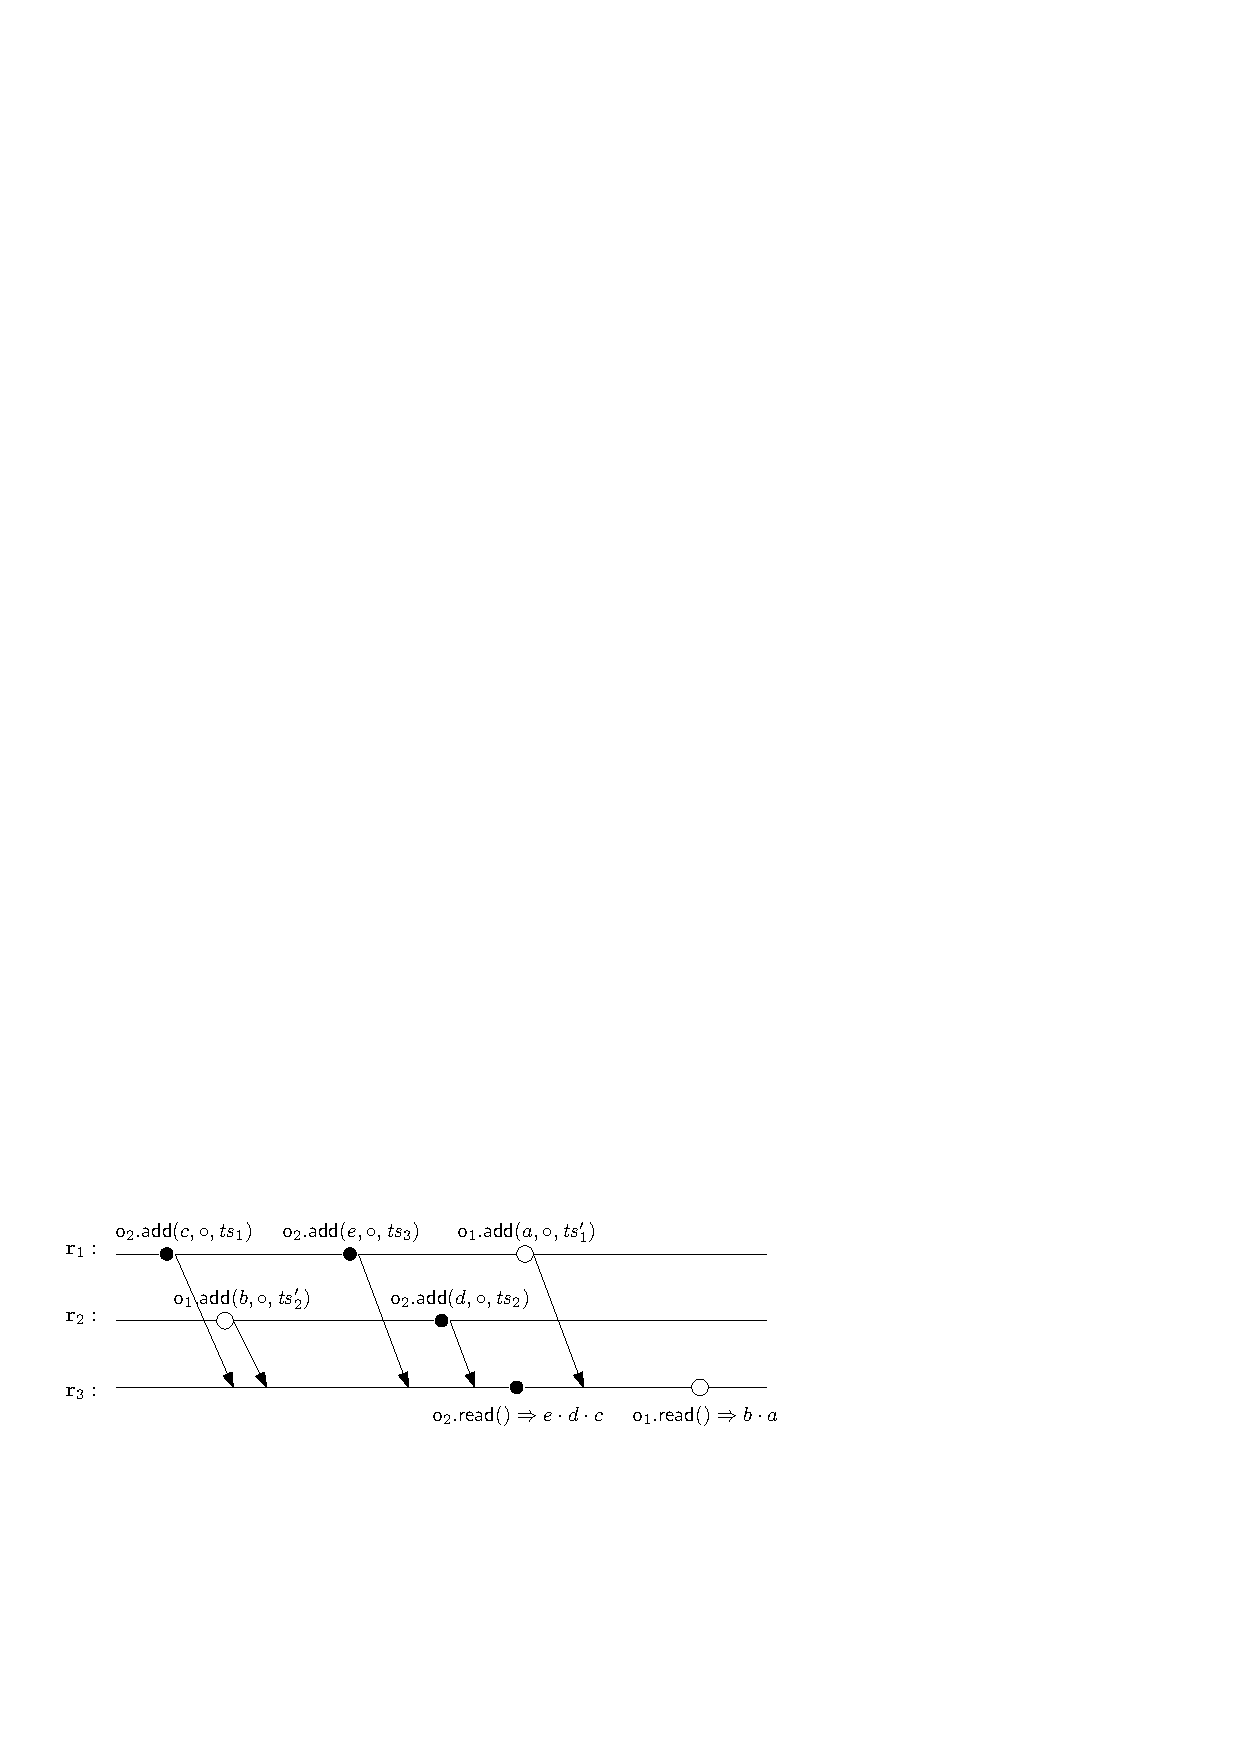
\includegraphics[width=0.7 \textwidth]{figures/LWWReg-LWWReg-NoSTS.pdf}
\vspace{-10pt}
  \caption{A failed example of composing two \tonelinearizable list object $\aobj_1$ and $\aobj_2$, where $\mathit{ts}_1 < \mathit{ts}_2 < \mathit{ts}_3$, and $\mathit{ts}'_1 < \mathit{ts}'_2$.}
  \label{fig:a failed example of composing two last-write-win registers}
\end{figure}


%To get rid of such problem, we require a condition called causal-timestamp. Intuitively, causal-timestamp requires multiple objects to ``share timestamp''. Formally, a history $\ahis$ satisfies causal-time-stamp, if for operations $\aop_1,\aop'_1,\ldots,\aop_k,\aop'_k$ of $\ahis$ satisfies the following condition, we have that the timestamp of $\aop'_1$ is less than that of $\aop_1$:

%\begin{itemize}
%\setlength{\itemsep}{0.5pt}
%\item[-] $(\aop_1,\aop'_1)$ are of a same object, $\ldots$, $(\aop_k,\aop'_k)$ are of a same object,

%\item[-] The timestamp of $\aop_2$ is less than that of $\aop'_2$, $\ldots$, the timestamp of $\aop_k$ is less than that of $\aop'_k$,

%\item[-] $(\aop'_1,\aop_2), \ldots, (\aop'_{\mathit{k-1}},\aop_k), (\aop'_k,\aop_1) \in \avisord{}$.
%\end{itemize}

To get rid of such problem, we additionally require that $(<_{\mathit{ts}} \cup \avisord)^*$ be acyclic. Here $<_{\mathit{ts}}$ is the order of timestamp for each object $\aobj$ where $\ahis \uparrow_{\aobj}$ is \tonelinearizable{} w.r.t its corresponding sequential specification. The following lemma states that, this condition is enough to deal with the case when there is more than one \tonelinearizable{} objects. Its proof can be found in Appendix \ref{subsec:appendix proofs of lemma several t0-specifications and several t1-specification can be composed}.

\begin{restatable}{lemma}{composingTZeroAndTOne}
\label{lemma:several t0-specifications and several t1-specification can be composed}
Given a multi-object history $\ahis$ satisfies acyclic $(<_{\mathit{ts}} \cup \avisord)^*$. If for each object $\aobj$, $\ahis \uparrow_{\aobj}$ is either \tzerolinearizable{} or \tonelinearizable{}, then, $\ahis$ is \crdtlinearizable{}.
\end{restatable}

The proof of this lemma is similar to that of Lemma \ref{lemma:several t0-specifications and one t1-specification can be composed}: We construct a \crdtlinearization of $h$ step by step by always choosing either an operation of a \tzerolin{} object that is minimal w.r.t $\avisord$, or an operation of a \tonelin{} object that is minimal w.r.t $\avisord$ and timestamp order. The condition of $(<_{\mathit{ts}} \cup \avisord)^*$ being acyclic will be used to prove that such process terminates with all operations of $\ahis$ put in the \crdtlinearization. \figurename~\ref{fig:compose two list} shows an successful example of composing two \tonelinearizable list object $\aobj_1$ and $\aobj_2$. As discussed above, in constructing the \crdtlinearization, in the first round, the only candidate is $\aobj_2.\mathit{add}(c,\circ)$; in the second round, the only candidate is $\aobj_1.\mathit{add}(a,\circ)$; in the third round, we could randomly choose $\aobj_1.\mathit{add}(b,\circ)$, and in the last round, we choose $\aobj_2.\mathit{add}(d,\circ)$. It is obvious that  $\aobj_2.\mathit{add}(c,\circ) \cdot \aobj_1.\mathit{add}(a,\circ) \cdot \aobj_1.\mathit{add}(b,\circ) \cdot \aobj_2.\mathit{add}(d,\circ)$ is the \crdtlinearization of the whole history.

\begin{figure}[t]
  \centering
  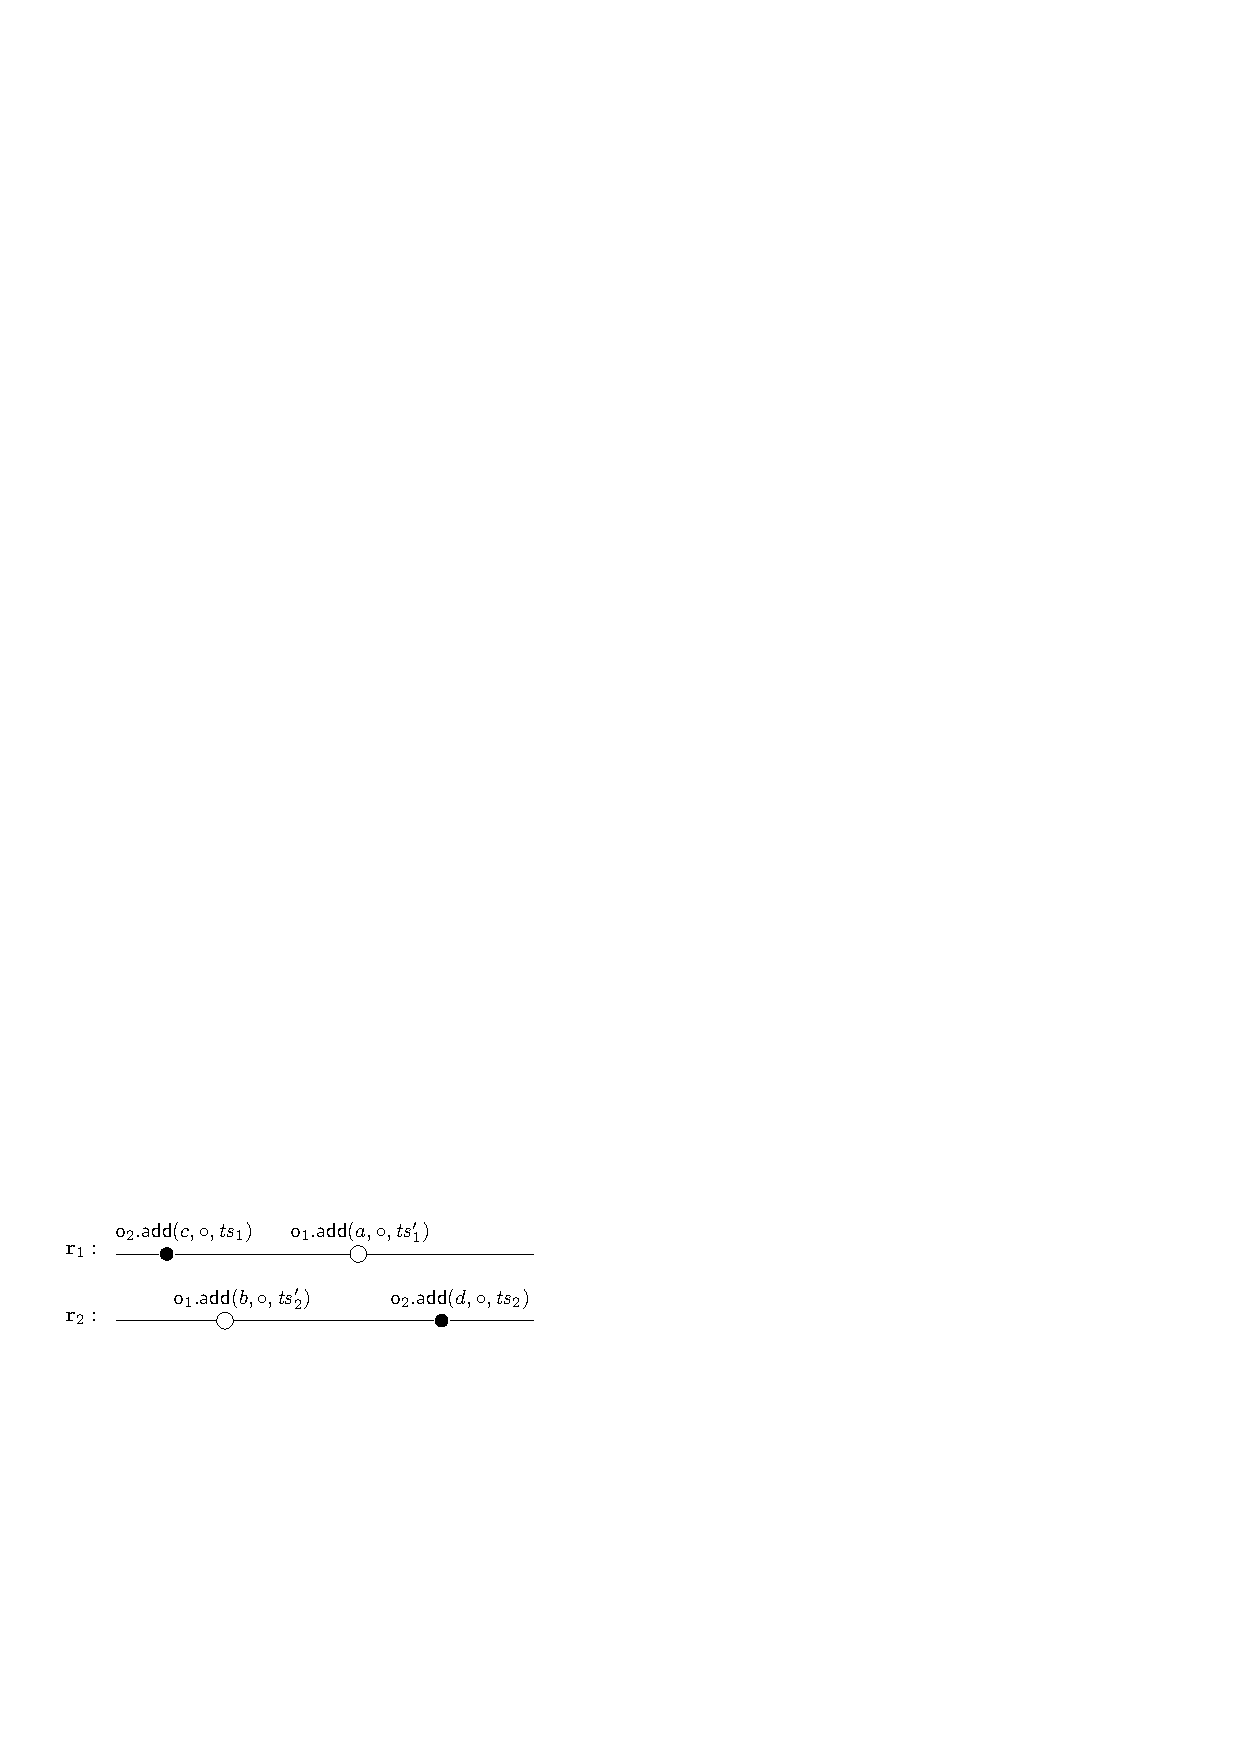
\includegraphics[width=0.45 \textwidth]{figures/Compose-TwoList.pdf}
\vspace{-10pt}
  \caption{A successful example of composing two \tonelinearizable list object $\aobj_1$ and $\aobj_2$, where $\mathit{ts}_1 < \mathit{ts}_2$, and $\mathit{ts}'_1 < \mathit{ts}'_2$.}
  \label{fig:compose two list}
\end{figure}

%Note that here we permit different \crdtimp{} to use different style of timestamp and order.





\subsection{Modified Implementation and Multi-Objects Semantics}
\label{subsec:smodified implementation and multi-objects semantics}

Given a set of objects, we may choose some objects which later will be proved to be ``\tzerolinearizable{}'' while other objects will be proved to be ``\tonelinearizable{}''. We may call the former objects and latter objects objects of \tzerolin{} and \tonelin{}, respectively.

To ensure the acyclic $(<_{\mathit{ts}} \cup \avisord)^*$ of Lemma \ref{lemma:several t0-specifications and several t1-specification can be composed}, we propose a semantics for multiple objects. %The transitive visibility can be easily satisfied by always choosing a minimum downstream w.r.t visibility relation among objects. To deal with causal-timestamp,
We introduce a \gts{} shared among objects of \tonelin{}. Objects of \tonelin{} use \gts{}, instead of its inner information, to generate new timestamp; The distributed system is responsible for updating global-timestamp, and we give only abstract restriction for it.

The value of \gts{} is a natural number $c \in \mathbb{N}$. The \gts{} have only one method called $\updategts{}$. $\updategts{}$ updates the value of \gts{} into a random bigger value and returns it. As discussed above, \crdtimp{} of objects of \tonelin{} is modified as follows: When we need to generate a new timestamp, we use method $\updategts{}$ to generate new timestamp. As an example, the modified RGA algorithm is shown in \autoref{lst:modified rga}. We can see that only line $7$ is modified.

\begin{lstlisting}[caption={Pseudo-code of the Modified RGA}, captionpos=b,label={lst:modified rga}]
  payload Ti-Tree N, Set Tomb
  initial N = @|$\emptyset$|@, Tomb = @|$\emptyset$|@

  addAfter(a,b) :
    atSource :
      precondition : b = @|$\circ$|@ or (b != @|$\circ$|@ and (b,_,_) @|$\in$|@ N and b @|$\not\in$|@ Tomb)
      let ts@|$_{\mathtt{a}}$|@ = @|$\updategts{}()$|@
      let ts@|$_{\mathtt{b}}$|@ = (b == @|$\circ$|@)?(0,r@|$_{0}$|@):(timestamp of b in N)
    downStream(a, ts@|$_{\mathtt{a}}$|@, ts@|$_{\mathtt{b}}$|@) :
      precondition: b = @|$\circ$|@ or (b != @|$\circ$|@ and (b, ts@|$_{\mathtt{b}}$|@,_) @|$\in$|@ N)
      N = N ts@|$\cup$|@ {(a, ts@|$_{\mathtt{a}}$|@, ts@|$_{\mathtt{b}}$|@)}

  remove(a) :
    atSource :
      precondition : a != @|$\emptyset$|@ and (a,_,_) @|$\in$|@ N and a @|$\notin$|@ Tomb
    downStream(a) :
      precondition : a != @|$\emptyset$|@ and (a,_,_) @|$\in$|@ N
      Tomb = Tomb @|$\cup$|@ {a}

  read() :
    return traverse(N, Tomb)
\end{lstlisting}

We use object with \gts{} to emphasize an object of \tonelin{} that uses $\updategts{}$ to generate new timestamp. Then, we could now introduce the semantics for multiple objects.

\begin{figure}[t]
  \centering

\begin{itemize}
\item $ \Theta \eqdef [\objs \rightarrow (\states \times \methods \times \datadomain  \rightarrow \datadomain \times \Delta \times \tss)] \ni \atsource$ \hspace{\fill} {\tt atSource}
\item $ \Delta \eqdef [\states \rightarrow \states] \ni \effector$ \hspace{\fill} {\tt downstream}
%\item $\semop[]{} : \labels \times \states \rightarrow (\states \rightarrow \states)$ \hspace{\fill} Operational Semantics of a Single Operation (Label)
\item $\localstates \eqdef \powerset{\labels} \times (\objs \rightarrow \states) \ni (\alabelset, \funobjtostates)$ \hspace{\fill} Local Configurations
\item $\globalstates \eqdef [\reps \rightarrow \localstates] \times \powerset{\labels \times \labels} \times [\labels \rightarrow \Delta] \ni (\gstates, \avisord, \downstreams )$ \hspace{\fill} Global Configurations
\end{itemize}


\[
  \inferrule[\text{\sc Operation}]
  {\gstates(\arep) = (\alabelset, \funobjtostates) \\ \atsource(\aobj)(\funobjtostates(\aobj), \amethod,\argv) = (\retv,\effector,\ats) \\  \effector(\funobjtostates(\aobj)) = \astate' \\ \alabel = \alabelobjind{\argv}{\retv}{(i,\ats)} \\ \mathit{unique}(i) }
  {(\gstates, \avisord, \downstreams) \xrightarrow{} (\gstates[\arep \leftarrow (\alabelset \cup \{\alabel\}, \funobjtostates[\aobj \rightarrow \astate'])], %\alabel
    \avisord \cup (\alabelset \times \{\alabel\}), \downstreams[\alabel \rightarrow \effector])}
\]


\[
  \inferrule[\text{\sc DownStream}]
  {\gstates(\arep) = (\alabelset, \funobjtostates) \\ \alabel \in \mathsf{min}_{\avisord}(\labeldom{\avisord} \setminus \alabelset) \\
    \downstreams(\alabel)= \delta \\ \alabel = \aobj.\_ \\ \delta(\funobjtostates(\aobj)) = \astate'}
  {(\gstates, \avisord, \downstreams) \xrightarrow{} (\gstates[\arep \leftarrow (\alabelset \cup \{\alabel\}, \funobjtostates[\aobj \rightarrow \astate'])], \avisord, \downstreams)}
\]

  \caption{Operational Semantics of multiple objects.}
  \label{fig:modified semantics for multiple object}
\end{figure}

Given a set $\severalobj$ of CRDT objects, where all objects of \tonelin{} are object with \gts{}, its semantics is defined as a transition system $\llbracket \severalobj \rrbracket_g = (\globalstates,\aglobalstate_0,\rightarrow)$ as in \figurename~\ref{fig:modified semantics for multiple object}, where $\globalstates$ is a set of global configurations, $\aglobalstate_0$ is the initial configuration, and $\rightarrow\subseteq \globalstates  \times \globalstates$ is the transition relation. The subscript $g$ represents \gts{}. The difference between $\llbracket \severalobj \rrbracket_g$ and $\llbracket \aobj \rrbracket$ is as follows:

In a local configuration $(\alabelset, \funobjtostates)$ of global configuration $(\gstates, \avisord, \downstreams)$, we use $\funobjtostates$ to store the states of objects. For some fixed initial replica state $\astate_0$, the initial global configuration is defined by $\aglobalstate_0 = (\gstates_0, \emptyset, \emptyset) \in \globalstates$, where $\gstates_0$ maps each replica $\arep$ into $(\emptyset, \funobjtostates_0)$, and $\funobjtostates_0$ maps each objects into its initial state.

In the first transition rule, we use the transition rule of object $\aobj$, and use the downstream to change the state of object $\aobj$ in local configuration of replica $\arep$. Note that here if $\aobj$ is an object of \tonelin{} and want to generate new timestamp, then method $\updategts$ is used to generate new timestamp. In the second transition rule, we choose a downstream $\effector$ that haven't been already executed at $\arep$ and is a minimal one with respect to the order $\avisord$ among such downstreams. Then we use $\effector$ to change the state of object $\aobj$ of local configuration of replica $\arep$, where $\aobj$ is the object of $\effector$.

Executions and reachable global configurations of $\llbracket \severalobj \rrbracket_g$ are defined as usual. $(\alabelset,\avisord)$ is a history of $\llbracket \severalobj \rrbracket_g$, if there exists an execution $e$ ending in a global configuration $(\gstates, \avisord, \downstreams)$, and the following conditions are satisfied: (1) each timestamp generated by calling $\updategts$ is unique, and (2) given operations $\alabel_1$ and $\alabel_2$ of objects of \tonelin{}, if they both use $\updategts$ to generate new timestamp and $(\alabel_1,\alabel_2) \in \avisord$, then the timestamp of $\alabel_1$ is less than that of $\alabel_2$. The set of histories $\histories(\severalobj)$ of objects $\severalobj$ is the set of histories of $\llbracket \severalobj \rrbracket_g$. Since all objects with \gts{} share a same timestamp generater, it is obvious that $(<_{\mathit{ts}} \cup \avisord)^*$ is acyclic. Note that, here we leave the way of implementing \gts{} completely abstract, and only give conditions to executions.

%In practice, one possible way to implement \gts{} is as follows:

%\begin{itemize}
%\setlength{\itemsep}{0.5pt}
%\item[-] Each replica stores a integer value $c$,
%\item[-] To do $\updategts$, returns $(c+1,\arep)$, and change $c$ into $c+1$, where $\arep$ is the identifier of current replica,
%\item[-] To do $\rupdategts$, returns $(c+d,\arep)$, and change $c$ into $c+s$, where $\arep$ is the identifier of current replica an $d$ is a random positive integer,
%\item[-] Embed $c$ in downstream of objects of \tonelin{},
%\item[-] When doing downstream, set value $c$ of current replica to be the maximum of current $c$ and the $c$ in downstream.
%\end{itemize}




\subsection{Composing Objects}
\label{lemma:composing objects}

%Given a object $\aobj$ with \gts{}, let $\mobj{\aobj}$ be an object obtained from $\aobj$ by using $\rupdategts$ instead of $\updategts$. It is obvious that, given a history $\ahis$ of $\llbracket \severalobj \rrbracket$, there is always a history $\ahis'$ of $\llbracket \mobj{\aobj} \rrbracket$, such that the projection of $\ahis$ into operations of $\mobj{\aobj}$ is $\ahis'$. To explain this, we can obtain an execution of $\ahis'$ from an execution of $\ahis$ by removing operations of other objects and use $\rupdategts$ instead of $\updategts$ to obtain new timestamp.

According to Lemma \ref{lemma:several t0-specifications and several t1-specification can be composed}, we have the first version of composing objects: Given a set $\severalobj$ of objects, if

\begin{itemize}
\setlength{\itemsep}{0.5pt}
\item[-] for each object $\aobj$ of \tzerolin{}, each history of $\llbracket \aobj \rrbracket$ is \tzerolinearizable{}
\item[-] for each object $\aobj$ of \tonelin{}, each history of $\llbracket \{ \aobj \} \rrbracket_g$ is \tonelinearizable{}
\end{itemize}

Then, each history of $\llbracket \severalobj \rrbracket_g$ is \crdtlinearizable{}. This holds since given a history $\ahis$ of $\llbracket \severalobj \rrbracket_g$ and an object $\aobj \in \severalobj$, $\ahis \uparrow_{\aobj}$ is a history of $\llbracket \aobj \rrbracket$ or $\llbracket \{ \aobj \} \rrbracket_g$. Recall that $\updategts$ increase into a random new value.

Although this gives an approach for modular proof, it is complex to prove \tzerolin{} or \tonelin{} for each object. Another problem is that we can not directly reuse our proof with execution-order simulation relation and timestamp-order simulation relation. We solve these problem by considering properties of sequential specifications.

We do not directly prove \tzerolin{}, but prove \crdtlinearizable{} w.r.t a \tzerospec{} instead. The notion \tzerospec{} is defined as follows:

\begin{definition}[\tzerospec{}]
\label{definition:t0-specification}
A sequential specification $\Spec$ is called a \tzerospec{}, if given a history $\ahis$ that is \crdtlinearizable{} w.r.t $\Spec$, then each specification sequence $(\alabelset, \aseqord)$ consistent with visibility order is a \crdtlinearization{}.
\end{definition}

The following lemma shows some sequential specifications are \tzerospec{}. Its proof can be found in Appendix \ref{subsec:appendix proofs of Lemma several t0-specifications}.

\begin{restatable}{lemma}{SeveralTZeroSpecifications}
\label{lemma:several t0-specifications}
$\mathit{OR}$-$\mathit{set}_s$, $\mathit{set}_s$ and $\mathit{counter}_s$ are \tzerospec{}.
\end{restatable}

Since the execution-order simulation relation uses a \crdtlinearization that consistent with visibility relation, it is obvious that, once we prove that $\aobj$ is \crdtlinearizable{} w.r.t a \tzerospec{} $\Spec$ by proving execution-order simulation relation, then, we know that $\aobj$ is \tzerolinearizable w.r.t $\Spec$.

Similarly, we do not directly prove \tonelin{}, but prove \crdtlinearizable{} w.r.t a \tonespec{} instead. The notion \tonespec{} is defined as follows:

\begin{definition}[\tonespec{}]
\label{definition:t1-specification}
A sequential specification $\Spec$ is called a \tonespec{}, if given a history $\ahis$ that is \crdtlinearizable{} w.r.t $\Spec$ with a \crdtlinearization{} consistent with timestamp order, then each specification sequence $(\alabelset, \aseqord)$ consistent with visibility order and timestamp order is a \crdtlinearization{}.
\end{definition}

The following lemma shows some sequential specifications are \tonespec{}. Its proof can be found in Appendix \ref{subsec:appendix proofs of Lemma several t1-specifications}.

\begin{restatable}{lemma}{SeveralTOneSpecifications}
\label{lemma:several t1-specifications}
$\mathit{list}_s^{\mathit{af}}$ and $\mathit{reg}_s$ are \tonespec{}.
\end{restatable}

Since the timestamp-order simulation relation uses a \crdtlinearization that consistent with visibility order and and timestamp order, it is obvious that, once we prove that each history of $\llbracket \mobj{\aobj} \rrbracket$ is \crdtlinearizable{} w.r.t a \tonespec{} $\Spec$ by proving timestamp-order simulation relation, then, we know that $\aobj$ is \tonelinearizable w.r.t $\Spec$.

Since previously when we prove \crdtimp using timestamp-order simulation relation, our prove does not rely on the detailed value of timestamp, and permit each new timestamp be a random larger timestamp. From our proof for these \crdtimp it is easy to obtain the proof for their modified version with \gts{}, and the proof can be found in Appendix \ref{a}.



\begin{table}
  \centering
  \begin{tabular}[t]{l|l}
    T0 & $\mathit{OR}$-$\mathit{set}_s$, $\mathit{set}_s$, $\mathit{counter}_s$,  \\
    T1 & $\mathit{list}_s^{\mathit{af}}$, $\mathit{reg}_s$,
  \end{tabular}
\end{table}

With these results, we finally have the following composing theorem.

\begin{theorem}[compositional theorem]
\label{definition:compositional theorem}
Given a set $\severalobj$ of objects, if

\begin{itemize}
\setlength{\itemsep}{0.5pt}
\item[-] For some object $\aobj$, each history of $\llbracket \{ \aobj \} \rrbracket_g$ is \crdtlinearizable{} w.r.t a \tonespec{} $\Spec$, and we prove by timestamp-order simulation relation.

\item[-] For other object $\aobj$, $\aobj$ is \crdtlinearizable{} w.r.t a \tzerospec{} $\Spec$, and we prove by execution-order simulation relation.
\end{itemize}

Then, each history of $\llbracket \severalobj \rrbracket_g$ is \crdtlinearizable{}.
\end{theorem}




\subsection{Tables and Graphs}
\label{lemma:tables and graphs}

{\color {red}CW: I put some tables and graphs here.}

{\color {red}CW: One question: Shapiro uses methods ``assign'' and ``value'' for register, while Burckhardt uses methods ``write'' and ``read''. Similarly, for set, Shapiro uses method ``lookup'' while Burckhardt uses ``read''.}

\figurename~\ref{fig:crdt-implementaton of this paper, their correctness, and their interface} gives the \crdtimp{} proved in our work, their correctness, and their interface (methods).

\begin{figure}[t]
  \centering

\begin{tabular}{|l|c|r|}
\hline
\crdtimp&Correctness&Interface\\
\hline
counter~\cite{ShapiroPBZ11}&\tzerolin&$inc$, $dec$\\
\hline
PN-counter~\cite{ShapiroPBZ11}&\tzerolin&$inc$, $dec$\\
\hline
LWW-register~\cite{?}&\tonelin&$write$, $read$\\
\hline
Multi-value register~\cite{?}&\tzerolin&$write$, $read$\\
\hline
2P-set~\cite{ShapiroPBZ11}&\tzerolin&$add$, $remove$, $read$\\
\hline
LWW-set~\cite{ShapiroPBZ11}&\tonelin&$add$, $remove$, $read$\\
\hline
PN-set~\cite{ShapiroPBZ11}&not \crdtlinearizable{}&$add$, $remove$, $read$\\
\hline
OR-set~\cite{ShapiroPBZ11}&\tzerolin&$add$, $remove$, $read$\\
\hline
RGA~\cite{?}&\tonelin&$addAfter$, $remove$, $read$\\
\hline
Wooki~\cite{?}&\tzerolin&$addBetween$, $remove$, $read$\\
\hline
Tree-Doc~\cite{?}&\tzerolin&$addBetween$, $remove$, $read$\\
\hline
\end{tabular}

\caption{\crdtimp{} of this paper, their correctness, and their interface.}
\label{fig:crdt-implementaton of this paper, their correctness, and their interface}
\end{figure}

\figurename~\ref{fig:how RGA works} gives a example that, if from one state we do concurrent $addAfter(b,c)$ and $addAfter(b,c)$, then it converges. If we then remove $b$, we just add it to tombstone.

\begin{figure}[t]
  \centering
  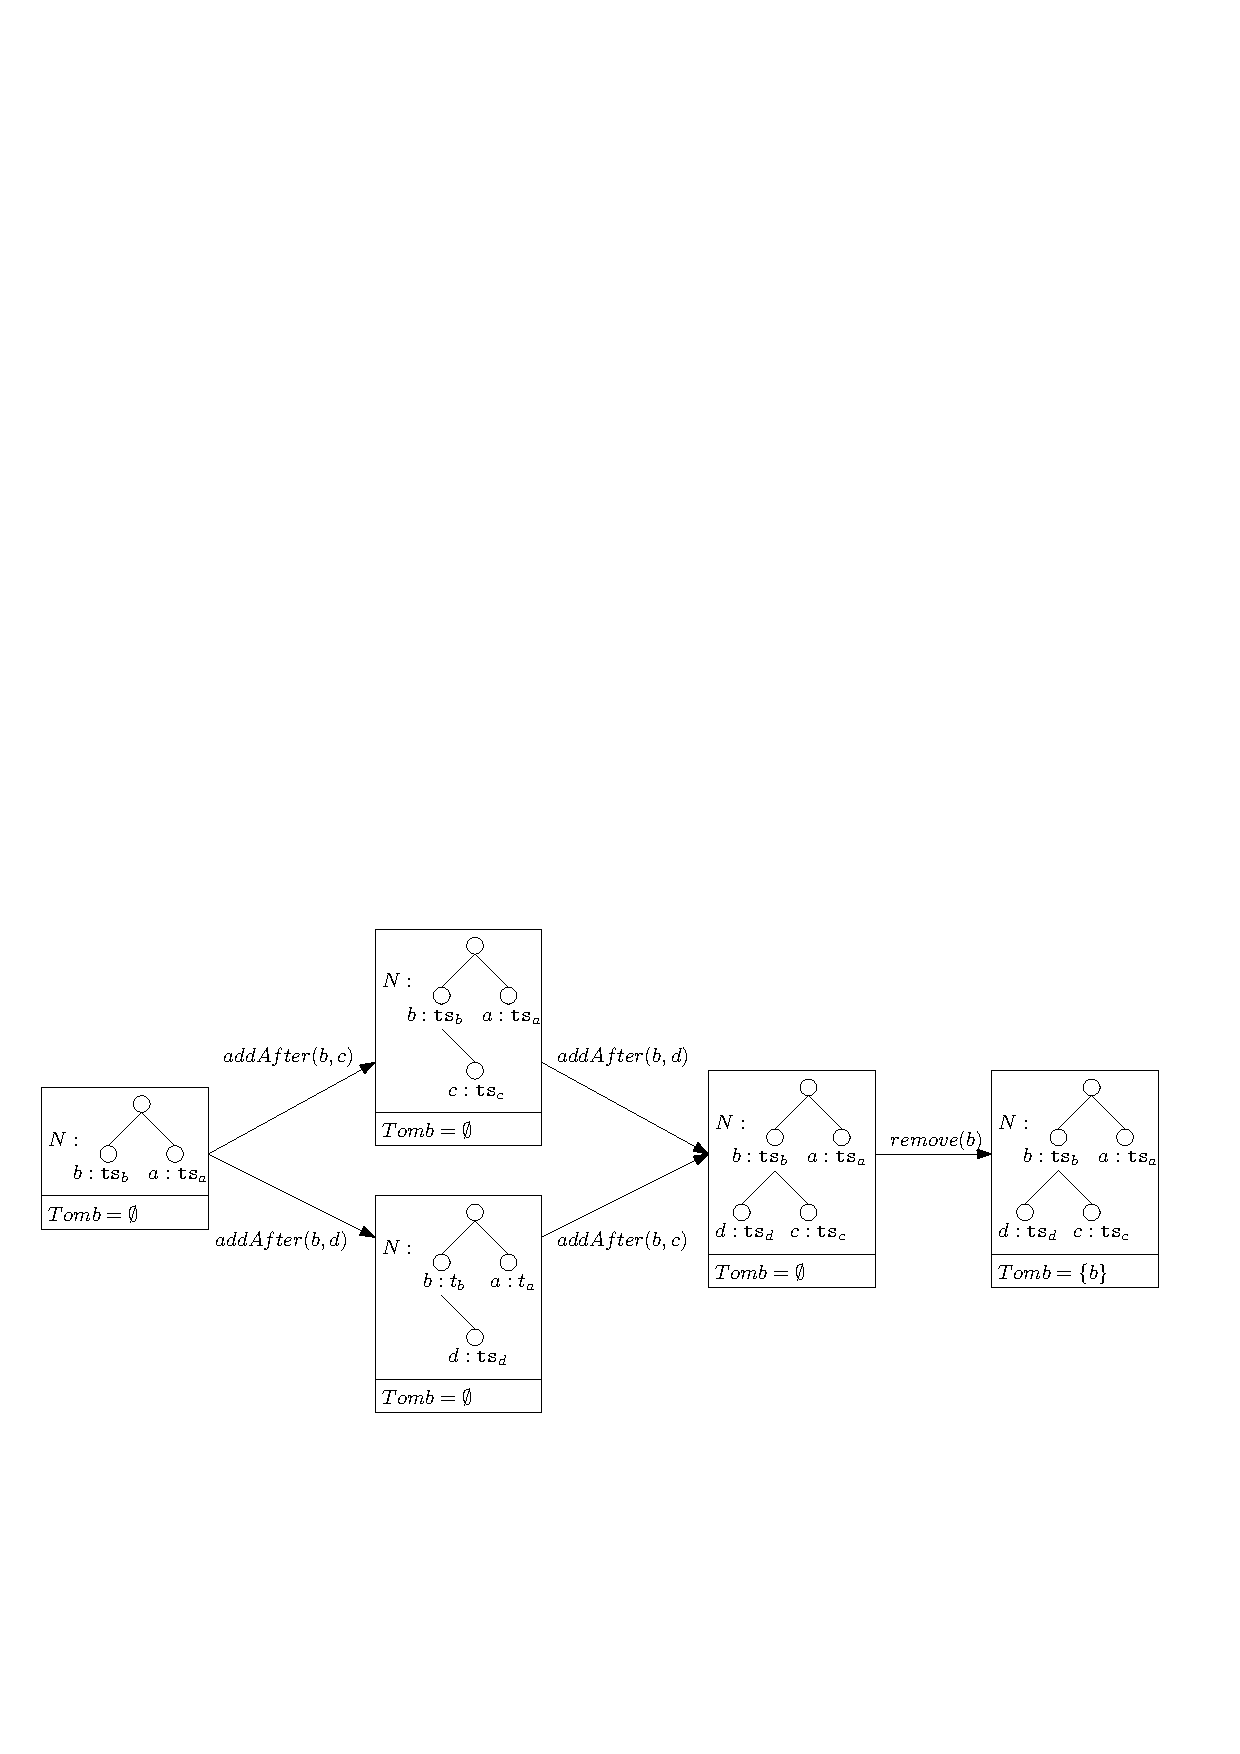
\includegraphics[width=0.85 \textwidth]{figures/HowRGAWork.pdf}
\vspace{-10pt}
  \caption{An example of conflict resolution of RGA, and how we do remove.}
  \label{fig:how RGA works}
\end{figure}


\figurename~\ref{fig:an example run of semantics} gives a example of two step of transitions on semantics of RGA. The first step is to do downstream of a $addAfter$, while the second step is to do operation $remove$. Here we can see that, the downstream of $addAfter$ always insert a new node into the Ti-tree $N$, while the downstream of $remove$ always insert a value into $Tomb$.

\begin{figure}[t]
  \centering
  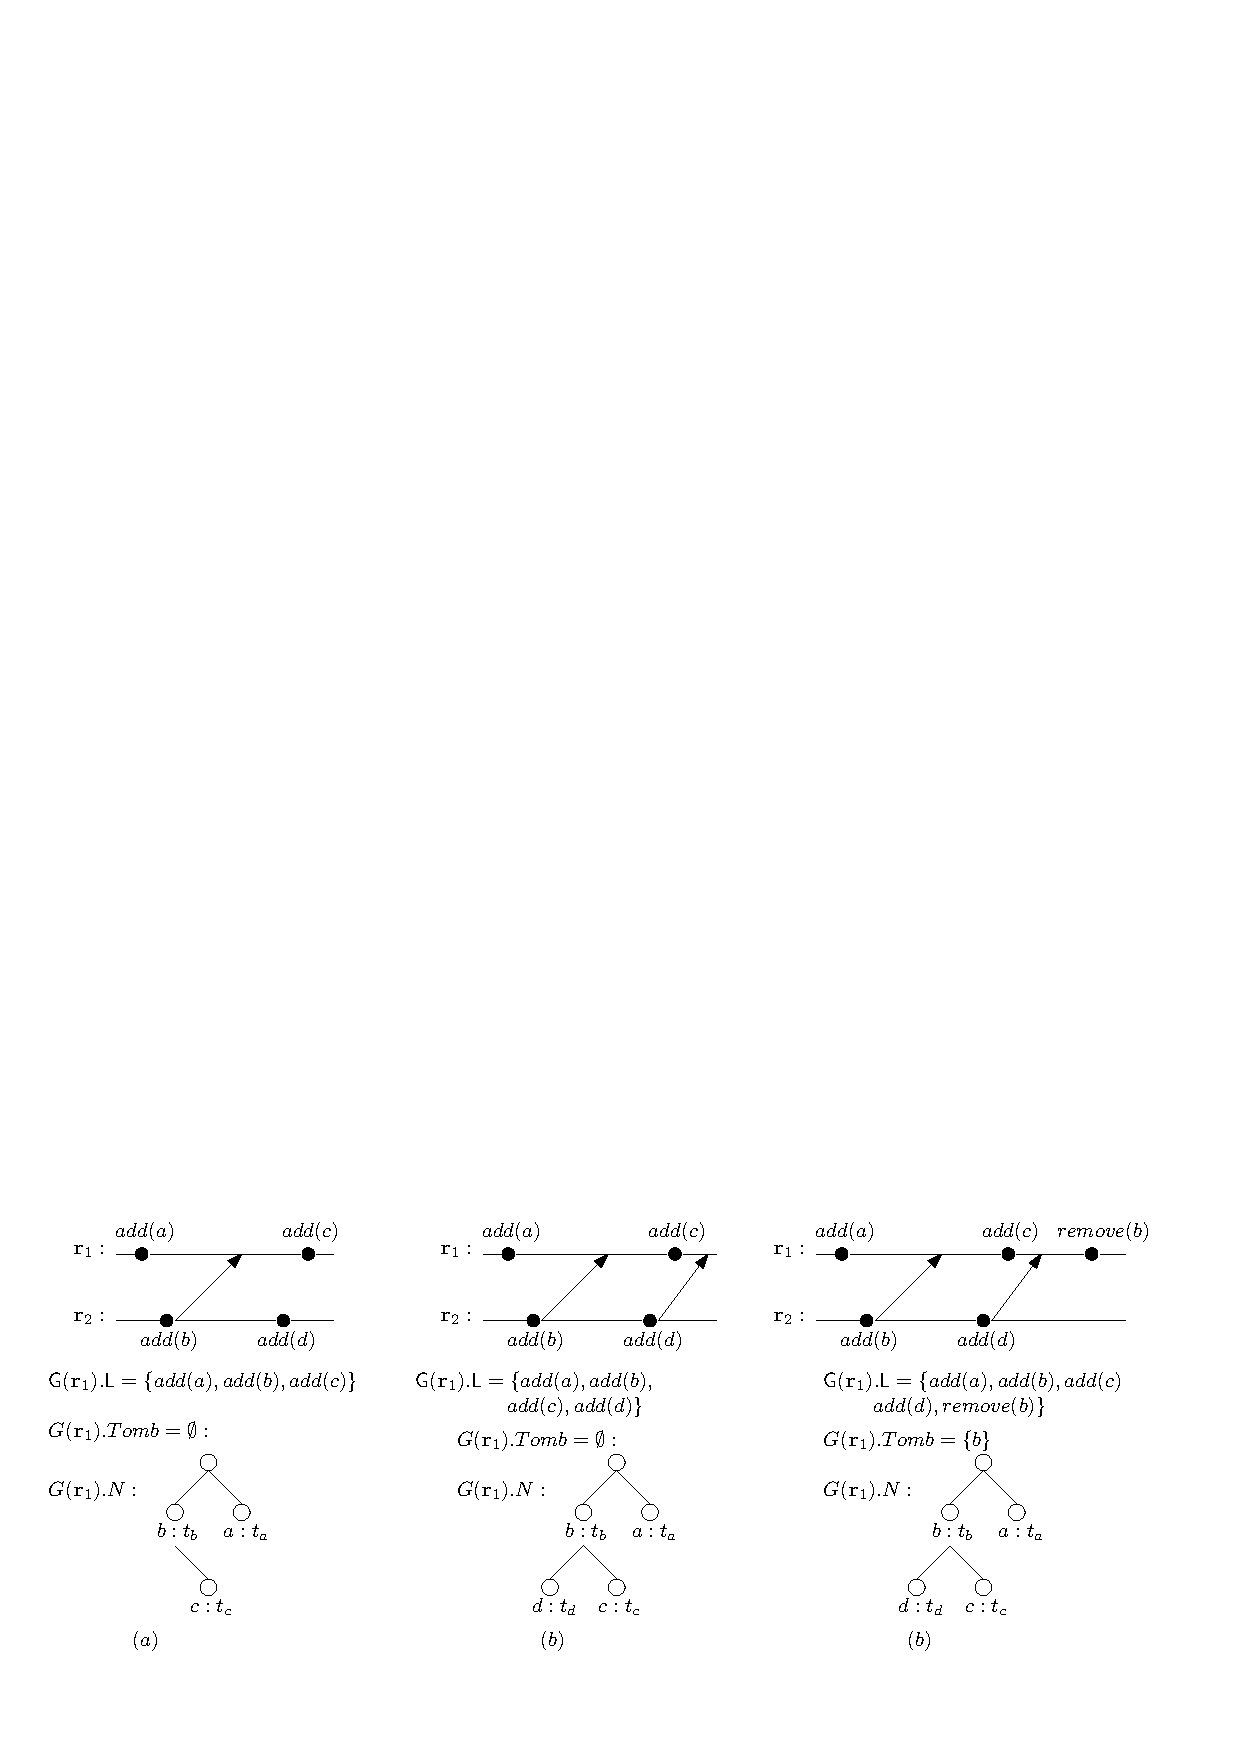
\includegraphics[width=0.9 \textwidth]{figures/ExplainSemantics.pdf}
\vspace{-10pt}
  \caption{An example run of semantics.}
  \label{fig:an example run of semantics}
\end{figure}


\figurename~\ref{fig:a history of RGA and its RA-linearization} gives a history of RGA and its \crdtlinearization{}. 

\begin{figure}[t]
  \centering
  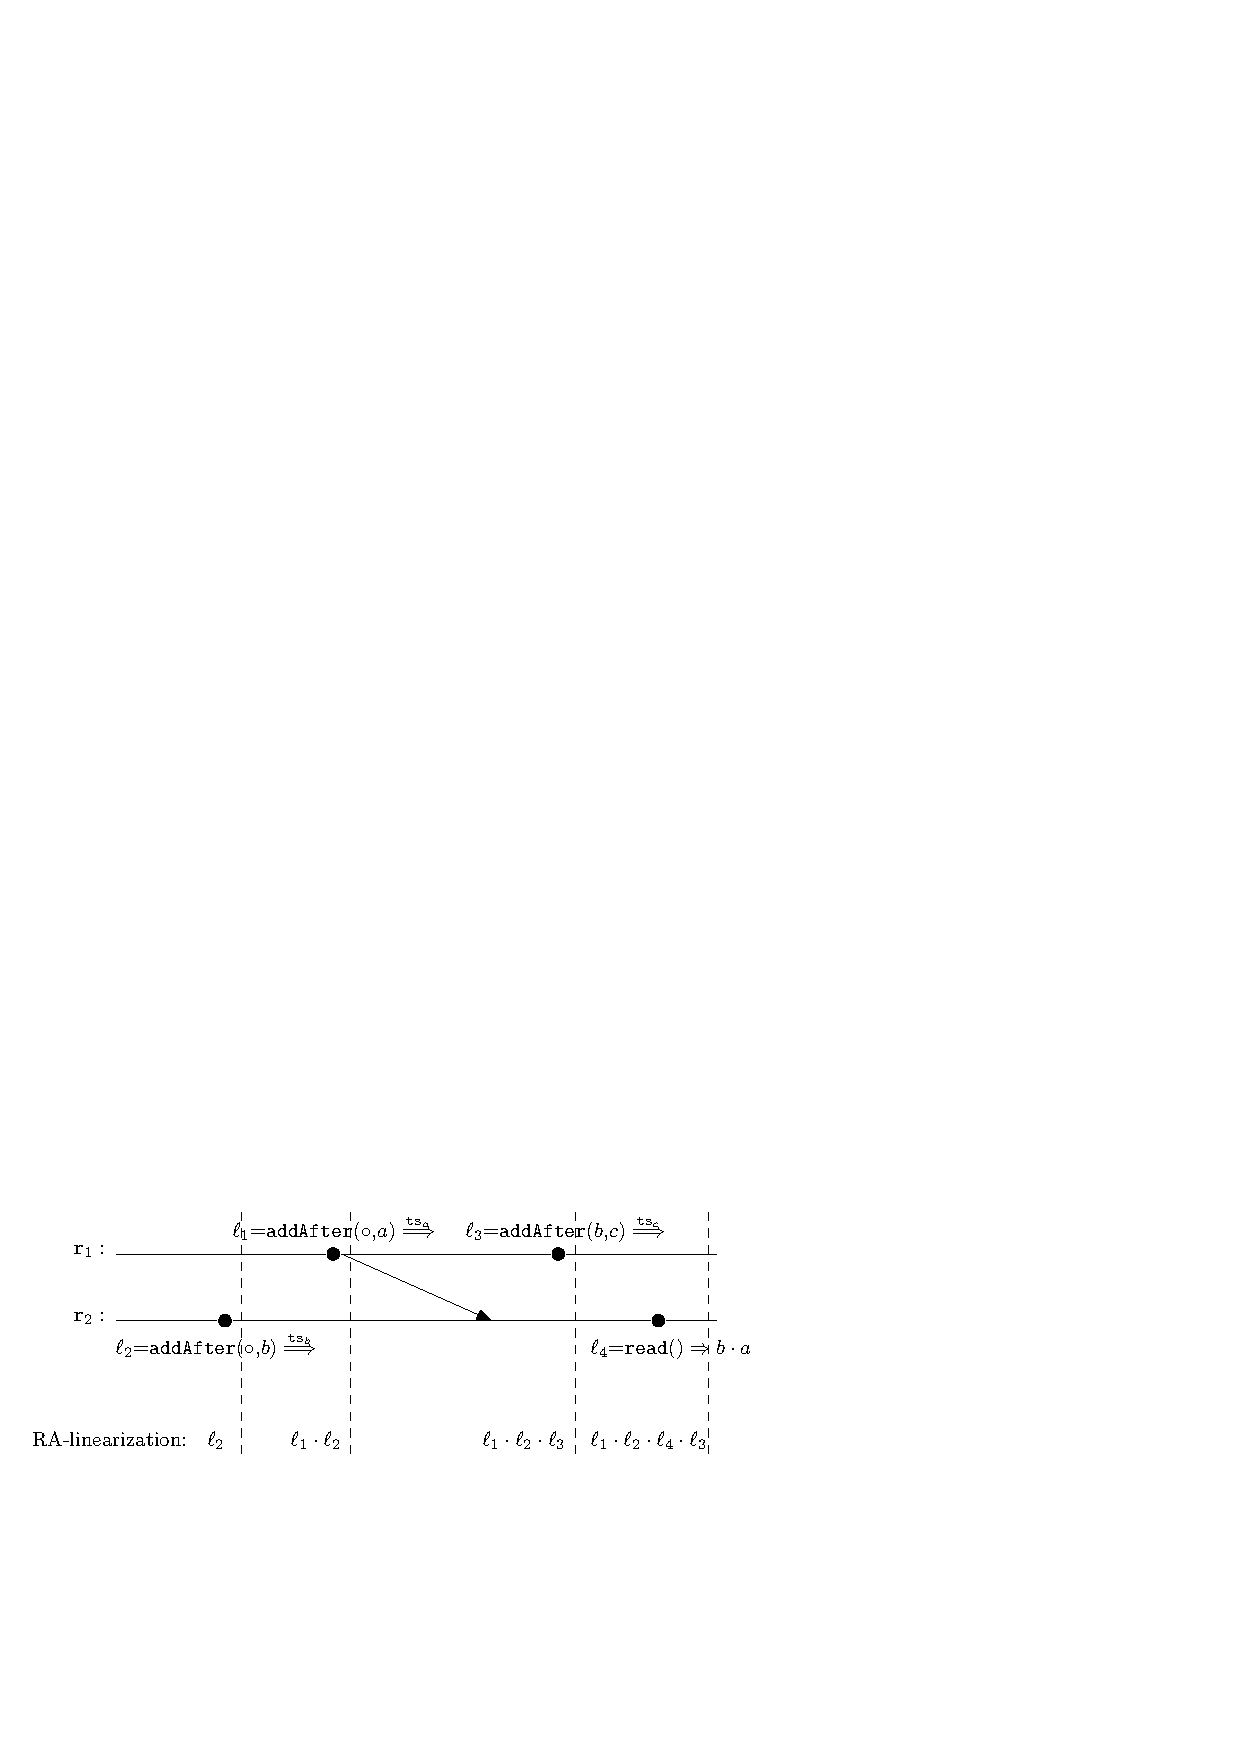
\includegraphics[width=0.6 \textwidth]{figures/RGAHisandLin.pdf}
\vspace{-10pt}
  \caption{A history of RGA and its \crdtlinearization{}.}
  \label{fig:a history of RGA and its RA-linearization}
\end{figure}


\figurename~\ref{fig:a history of OR-set, its update-query rewriting, and its RA-linearization} gives a history of OR-set, its query-update rewriting, and its \crdtlinearization{}.

\begin{figure}[t]
  \centering
  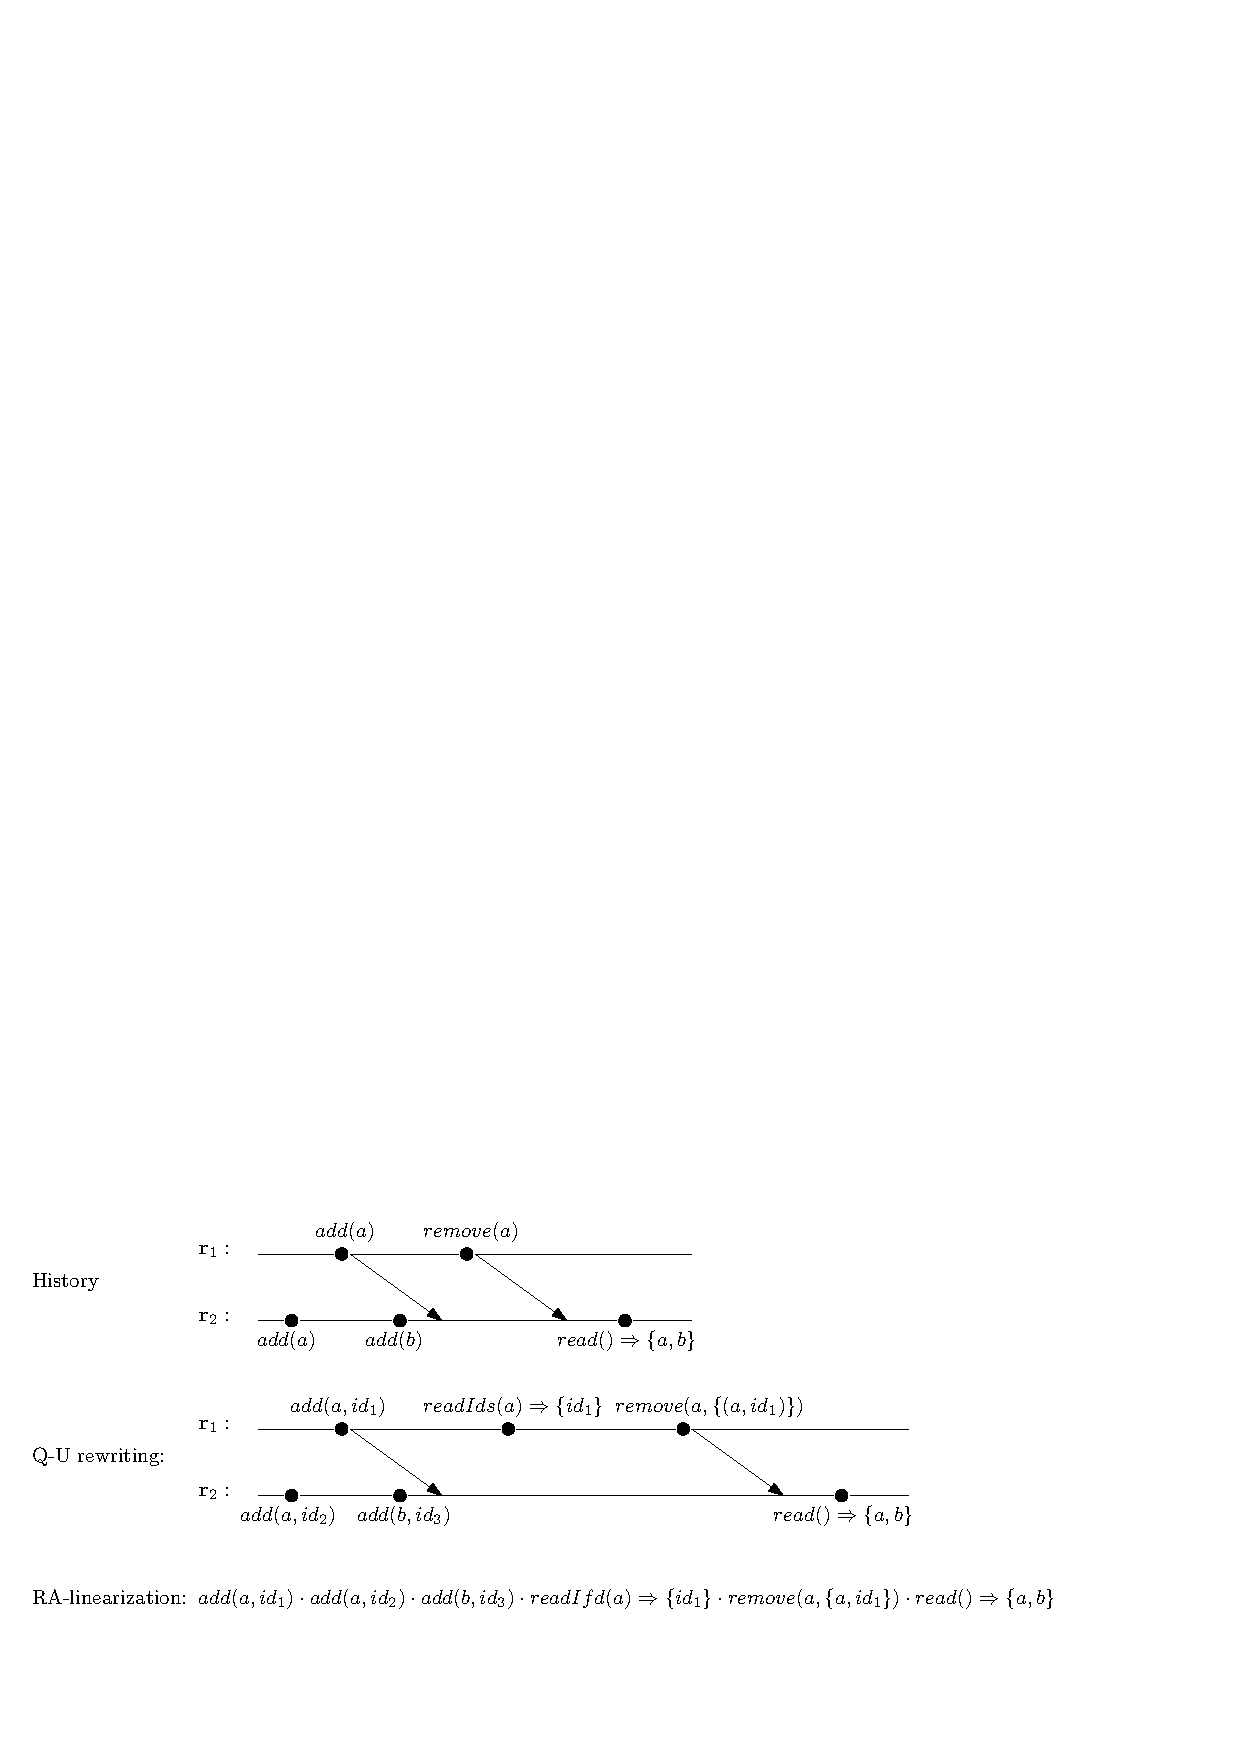
\includegraphics[width=0.8 \textwidth]{figures/ORSetHisRewritingandLin.pdf}
\vspace{-10pt}
  \caption{A history of OR-set, its update-query rewriting, and its \crdtlinearization{}.}
  \label{fig:a history of OR-set, its update-query rewriting, and its RA-linearization}
\end{figure}


\figurename~\ref{fig:how refinement mapping works} shows how refinement mapping works. \figurename~\ref{fig:how refinement mapping works} (a) shows the case of update labels, \figurename~\ref{fig:how refinement mapping works} (b) shows the case of query labels, and \figurename~\ref{fig:how refinement mapping works} (c) shows the case of update-query labels. 

Note that, in \figurename~\ref{fig:how refinement mapping works} (a) there is a ``gap'' between $\refmap(\sigma)$ and $\refmap(\sigma')$: it may be not the case that $\refmap(\sigma)\xRightarrow{\alabel}\refmap(\sigma')$. Although $\refmap(\sigma')$ should be obtained from $\refmap(\sigma_0)$ by a sequence of the same set of operations as from $\sigma_0$ to $\sigma'$, the order may be different. Such a transition exists for execution-order linearizations, and may not exist for timestamp-order linearizations. What we require here is only that the existence of $\refmap(\sigma')$.

\begin{figure}[t]
  \centering
  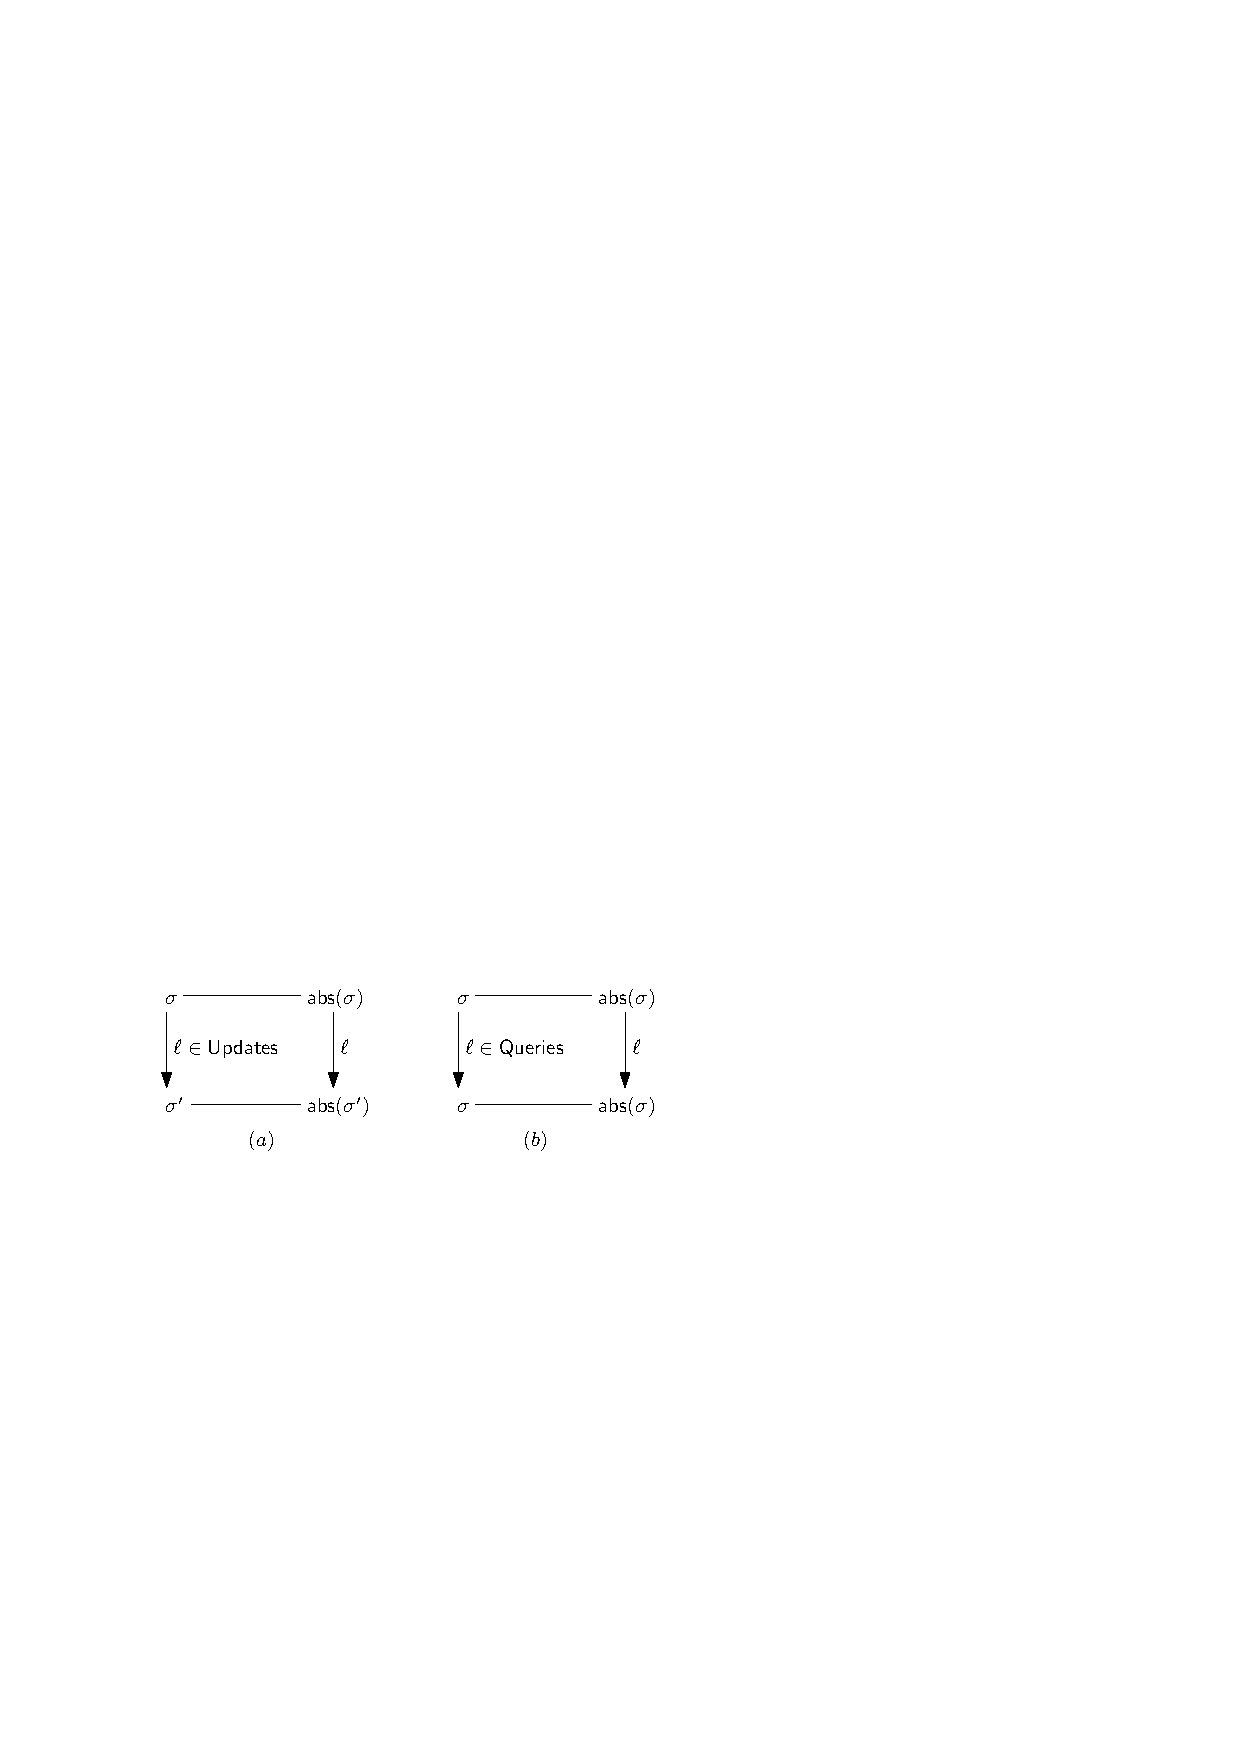
\includegraphics[width=0.8 \textwidth]{figures/RefinementMapping.pdf}
\vspace{-10pt}
  \caption{How refinement mapping works.}
  \label{fig:how refinement mapping works}
\end{figure}



\figurename~\ref{fig:an example of refinement mapping of an execution of RGA} gives an example of refinement mapping of an execution of RGA. Note that, there is a gap between $\refmap(\sigma_2)$ and $\refmap(\sigma_3)$. Or we can say that, the tansition $\refmap(\sigma_2)\xRightarrow{addAfter(\circ,a)}\refmap(\sigma_3)$ does not hold. 

\begin{figure}[t]
  \centering
  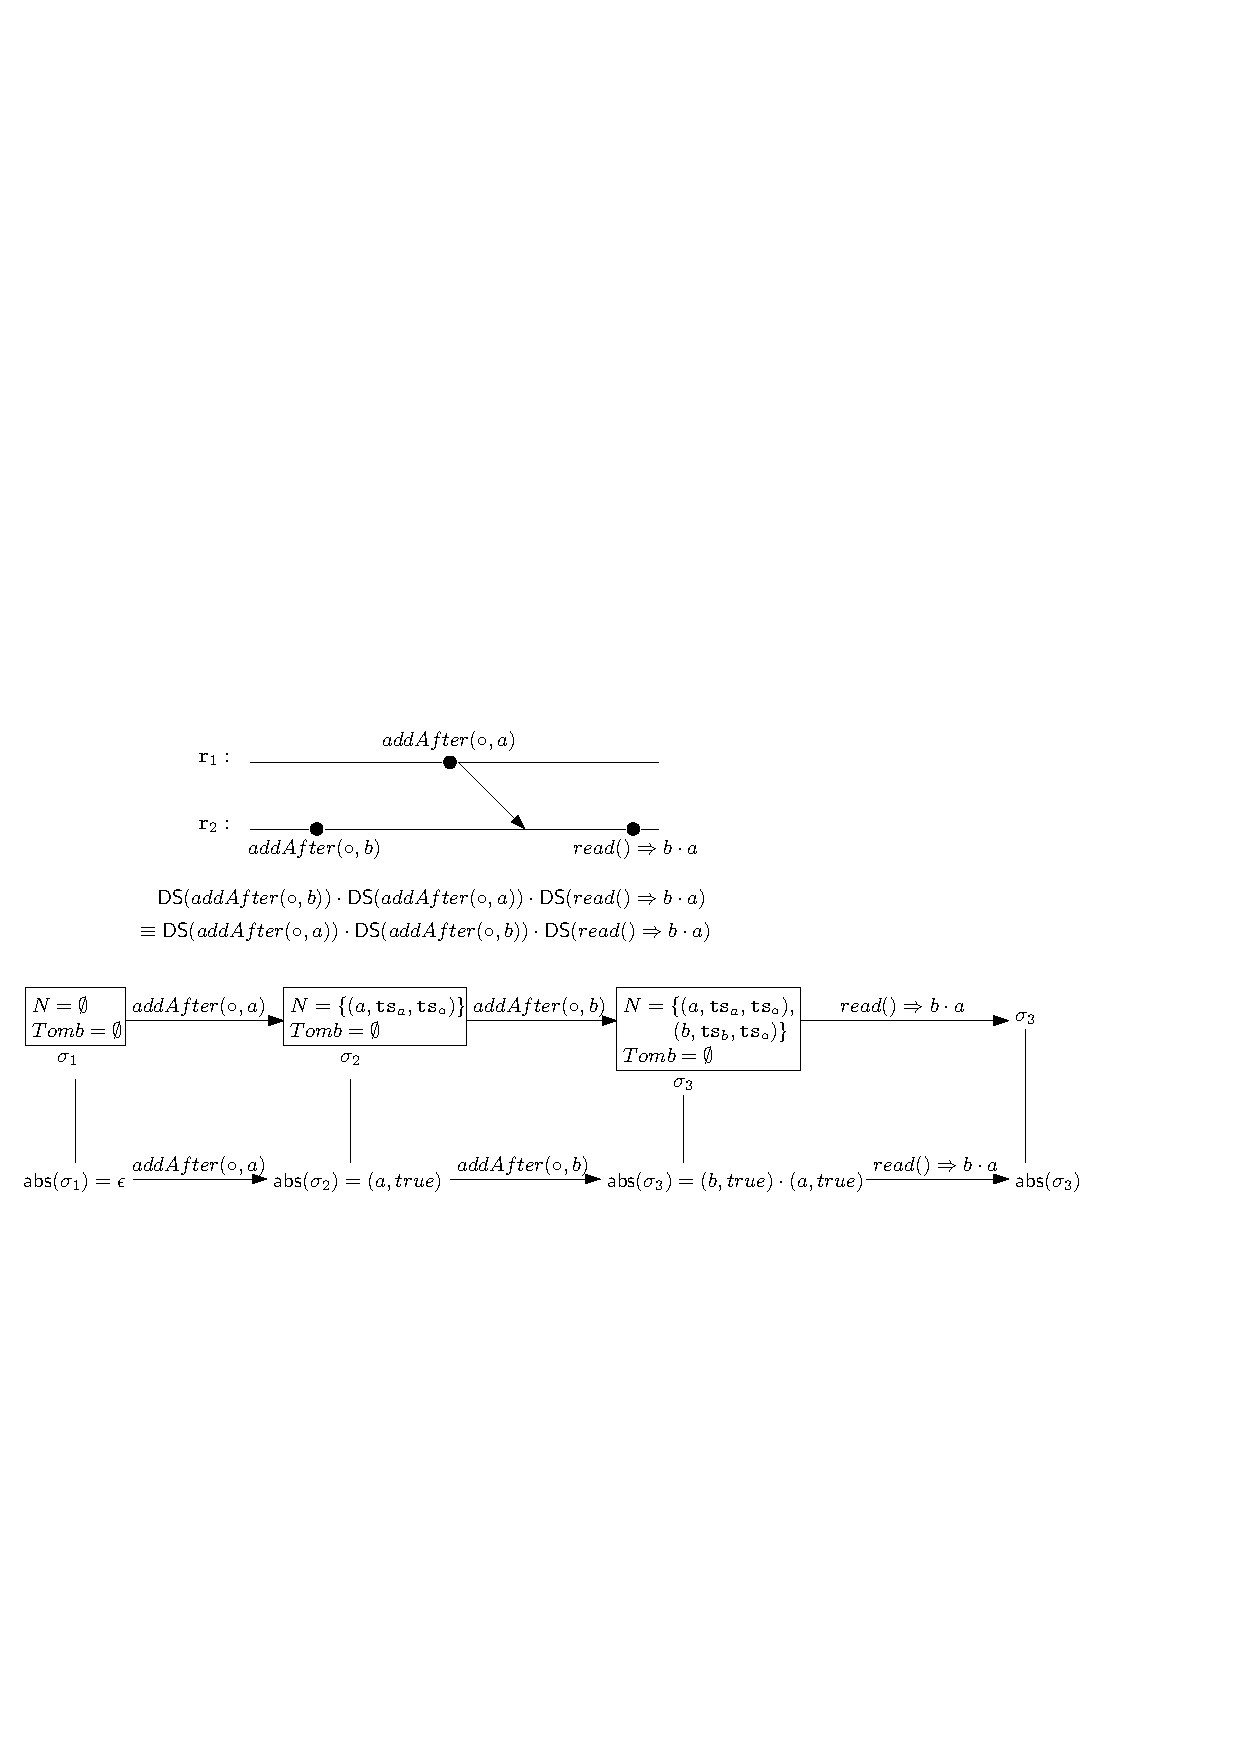
\includegraphics[width=0.85 \textwidth]{figures/RefinementMappingRGA.pdf}
\vspace{-10pt}
  \caption{An example of refinement mapping of an execution of RGA.}
  \label{fig:an example of refinement mapping of an execution of RGA}
\end{figure}



\figurename~\ref{fig:an example of refinement mapping of an execution of or-set} gives an example of refinement mapping of an execution of OR-set. Note that, there is no gap for OR-set, since it uses execution-order linearizations. 

\begin{figure}[t]
  \centering
  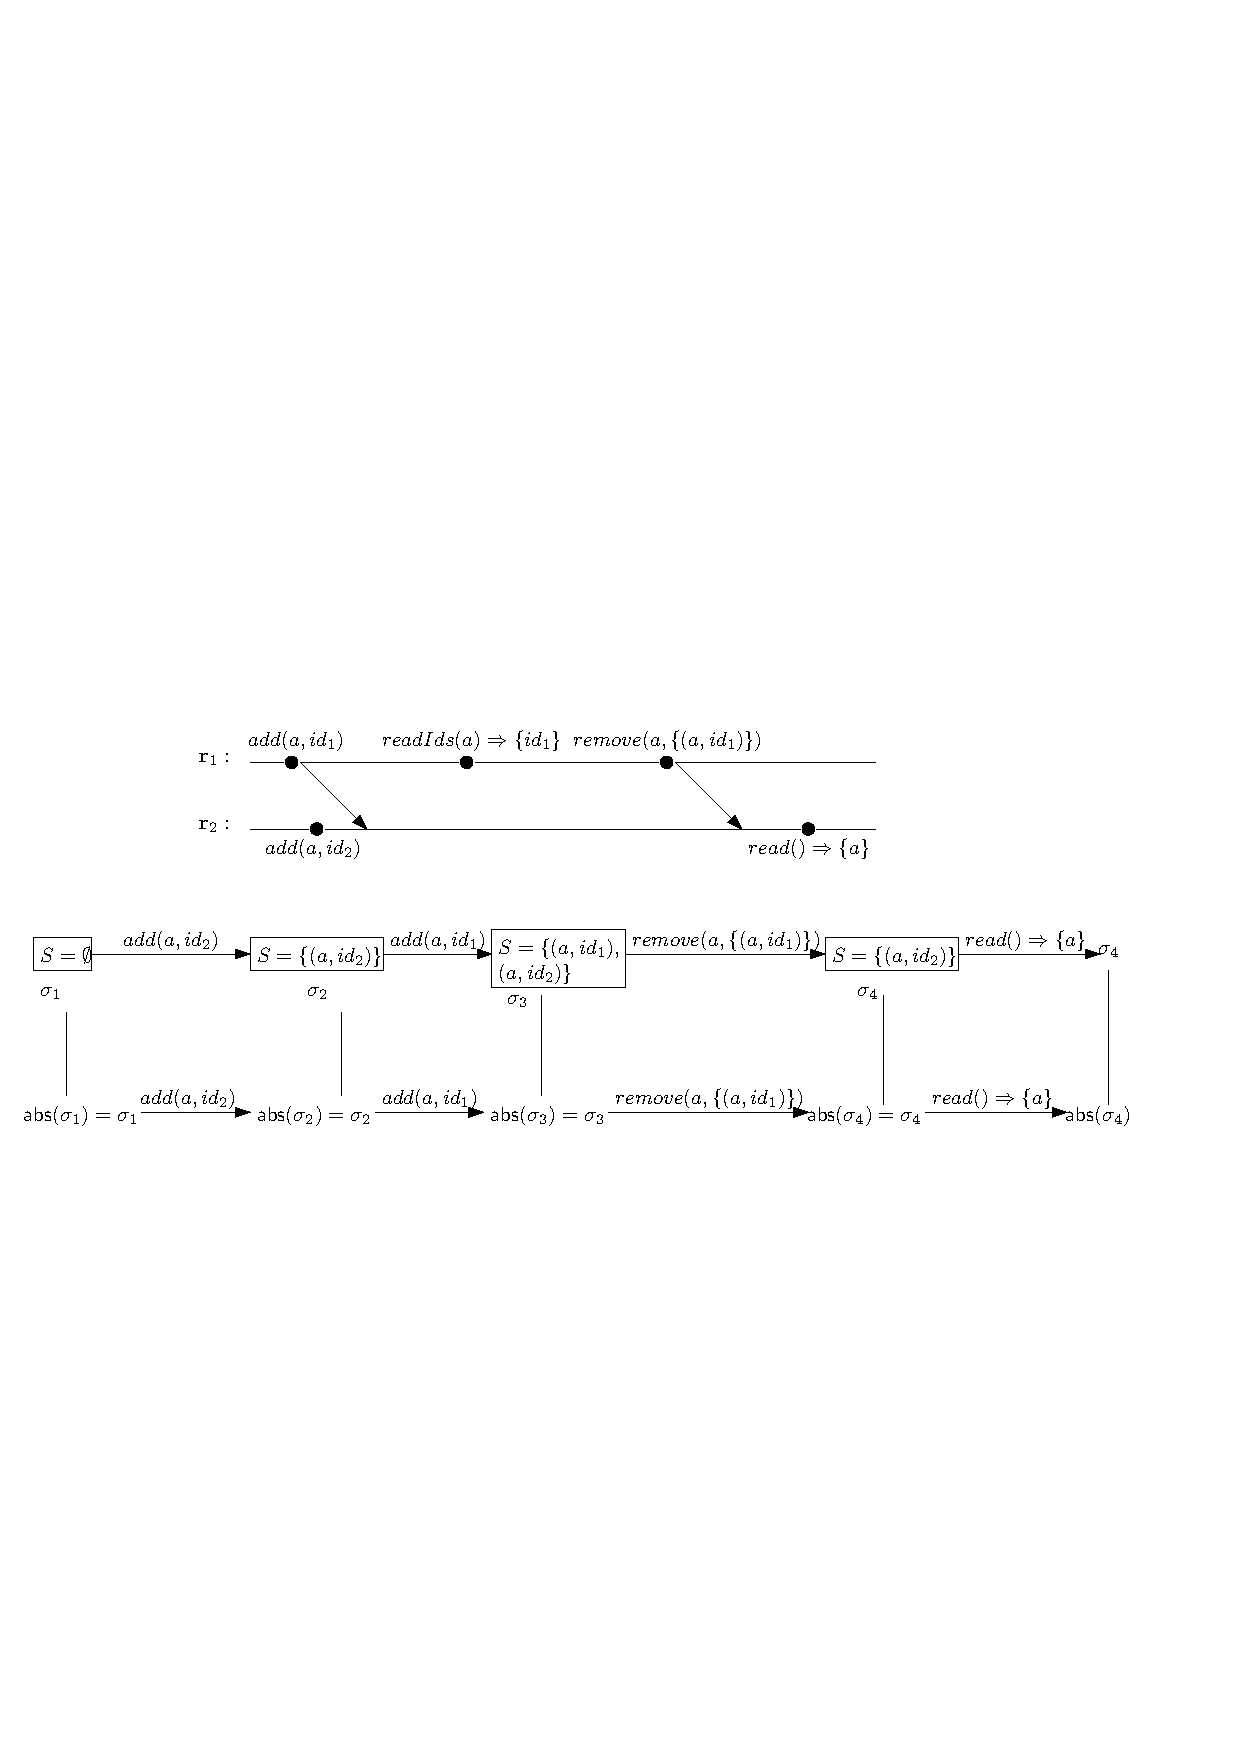
\includegraphics[width=0.85 \textwidth]{figures/RefinementMappingORSet.pdf}
\vspace{-10pt}
  \caption{An example of refinement mapping of an execution of OR-set.}
  \label{fig:an example of refinement mapping of an execution of or-set}
\end{figure}



The proof of $\mathsf{Refinement}$ relies on a \emph{refinement mapping}~\cite{AbadiL91} between replica states and states of the specification, denoted by $\refmap$. The proof goals require that for any two replica states $\sigma$ and $\sigma'$,
\begin{enumerate}
\item If $\sigma'$ is obtained from $\sigma$ by applying a downstream produced by an update $\alabel$: There exists a abstract $\refmap(\sigma')$ that is obtained from $\abstate_0$ by appling the downstreams of the operations in $\alabelset \cup \{ \alabel \}$ in the order defined by $\aseqord$. 
          
\item if a query $\alabel$ is applied on a state $\sigma$ or it is introduced by a rewriting of a query-update that executes {\tt atSource} on a state $\sigma$, then $\refmap(\sigma)\xRightarrow{\alabel}\refmap(\sigma)$. 
\end{enumerate}

For the case of execution-order linearizations, the first case can be simplified into 

\begin{enumerate}
\item if $\sigma'$ is obtained from $\sigma$ by applying a downstream $\delta$ produced by an update $\alabel$, then \mbox{$\refmap(\sigma)\xRightarrow{\alabel}\refmap(\sigma')$}, where $\xRightarrow{\alabel}$ is the transition function of $\Spec$. 
\end{enumerate}

This simplification relies on proving concurrent operations commute. 






























\forget{

\section{Compositionality of Distributed Linearizability}
\label{sec:compositionality of distributed linearizability}

\textblue{
This section should give three results of the form: if $o_1$ is linearizable w.r.t. $S_1$ and $o_2$ is linearizable w.r.t. $S_2$, and ???, then $o_1 \otimes o_2$ is linearizable w.r.t. $S_1\times S_2$ (the 2-object spec defined by interleavings). ??? may be an additional condition, while $\otimes$ is an "operator" for composing two CRDT implementations. Every result will have a different $\otimes$ operator.
\begin{itemize}
\item T0 + T0: ??? = $S_1$ and $S_2$ are $T0$-specs, and $\otimes$ is the trivial composition (the "unsynchronized" product)
\item T1 + T1: ??? = $S_1$ and $S_2$ are $T1$-specs, and $\otimes$ is the "shared counter" composition (the "unsynchronized" product with a restriction on the set of generated histories)
\item T0 + T1: ??? = $S_1$ is a $T_0$ spec, and $S_2$ is a $T1$-spec, and $\otimes$ is the "global causal delivery" composition (the "unsynchronized" product with a restriction on the set of generated histories)
\end{itemize}
Also, we should prove that composing two $T0$, resp., $T1$, specs results in a $T0$, resp., $T1$ spec, and composing a $T0$ with $T1$ results in a $T1$. With this, the extension to sets of objects is straightforward:  compose all $T0$ and independently, all $T1$, then compose the two resulting objects.}


\subsection{Definition of Compositionality}
\label{subsec:definition of compositionality}

The following is the definition of distributed linearizability for multi-object histories.

\begin{definition}[Distributed Linearizability for Multi-object Histories]
\label{definition:distributed linearizability for multi-object histories}
A multi-object history $h$ is \crdtlinearizable{}, if there exists a sequence $\mathit{lin}$, called linearization of $h$, such that

\begin{enumerate}[(i)]
\item The elements of $\mathit{lin}$ is generated from the operations of $h$: each operation $o = (m(a) \Rightarrow b,i,\mathit{obj})$ is transformed into $(m(a) \Rightarrow b,i,S)$ with $S$ set of identifiers of operations of visible to $o$ via $h.\mathit{vis}$.
\item $\mathit{lin}$ is consistent with $h. \mathit{vis}$.
\item For each object $\mathit{obj}$, $h \uparrow_{\mathit{obj}}$ is \crdtlinearizable{}, and $\mathit{lin} \uparrow_{ \mathit{obj} }$ is a \crdtlinearization{} of $h \uparrow_{\mathit{obj}}$.
\end{enumerate}

A set $H$ of multi-object histories are \crdtlinearizable{} w.r.t deterministic sequential specifications, if each of its history is.
\end{definition}

The following is the definition of compositional histories.

\begin{definition}[Compositionality]
\label{definition:compositionality}
A multi-object history $h$ is called compositional, if: $h \uparrow_{\mathit{obj}}$ is distributed linearizable for each object $\mathit{obj}$, if and only if, $h$ is distributed linearizable.
\end{definition}

It is easy to see that, a multi-object history $h$ being distributed linearizable implies that the projection of $h$ into each object is distributed linearizable. When proving compositionality, we only need to consider the opposite direction.




\subsection{T0-Linearizability and T1-Linearizability}
\label{subsec:t0-linearizability and t1-linearizability}

To prove compositional

T0-linearizability is a sub-class of distributed linearizability.

\begin{definition}[t0-linearizability]
\label{definition:t0-ilnearizability}
A single-object history $h$ is t0-linearizable w.r.t a sequential specification $\mathit{spec}$, if each sequence $\mathit{lin}$ shown below is a linearization of $h$ w.r.t $\mathit{spec}$:

\begin{itemize}
\setlength{\itemsep}{0.5pt}
\item[-] Each element $(\ell,i,\mathit{vis}^{-1}(i))$ of $\mathit{lin}$ is generated from an operation $(\ell,i,\_,\mathit{ts})$ of $h$.

\item[-] $\mathit{lin}$ is consistent with $\mathit{vis}$.
\end{itemize}
\end{definition}

To prove t0-linearizability, we introduce the notion of t0-specifications. A specification $\mathit{spec}$ is called t0-specification, if given a history $h$ that is distributed linearizable w.r.t $\mathit{spec}$, then any sequence that is consistent with visibility relation is a linearization of $h$.

The following lemma shows some sequential specifications are t0-specifications. Its proof can be found in Appendix \ref{subsec:appendix proofs of Lemma several t0-specifications}. Based on this lemma and our proofs in Section \ref{sec:proving distributed linearizability}, we can see that or-set is t0-linearizable w.r.t $\mathit{OR}$-$\mathit{set}_s$, and counter is t0-linearizable w.r.t $\mathit{counter}_s$.

\begin{restatable}{lemma}{SeveralTZeroSpecifications}
\label{lemma:several t0-specifications}
$\mathit{OR}$-$\mathit{set}_s$, $\mathit{set}_s$ and $\mathit{counter}_s$ are t0-specifications.
\end{restatable}



Given a history $h$, a sequence $\mathit{lin}$ is called a strict time-stamp order candidate of $h$, if for each elements $o_1,o_2$ of $\mathit{lin}$, if the time-stamp of $o_1$ in $h$ is less than that of $o_2$, then, $o_1$ is before $o_2$ in $\mathit{lin}$. T1-linearizability is a sub-class of distributed linearizability.

\begin{definition}[t1-linearizability]
\label{definition:t1-ilnearizability}
A single-object history $h$ is t1-linearizable w.r.t a sequential specification $\mathit{spec}$, if each strict time-stamp order candidiate $\mathit{lin}$ is a linearization of $h$.
\end{definition}

To prove t1-linearizability, we introduce the notion of t1-specifications. A specification $\mathit{spec}$ is called t1-specification, if given a history $h$ that is distributed linearizable w.r.t $\mathit{spec}$, and has a strict time-stamp order candidate as linearization, then any strict time-stamp order candidate is a linearization of $h$.

The following lemma shows some sequential specifications are t1-specifications. Its proof can be found in Appendix \ref{subsec:appendix proofs of Lemma several t1-specifications}. Based on this lemma and our proofs in Section \ref{sec:proving distributed linearizability}, we can see that RGA is t1-linearizable w.r.t $\mathit{list}_s^{\mathit{af}}$, and LWW-register is t1-linearizable w.r.t $\mathit{reg}_s$.

\begin{restatable}{lemma}{SeveralTOneSpecifications}
\label{lemma:several t1-specifications}
$\mathit{list}_s^{\mathit{af}}$ and $\mathit{reg}_s$ are t1-specifications.
\end{restatable}


\begin{table}
  \centering
  \begin{tabular}[t]{l|l}
    T0 & $\mathit{OR}$-$\mathit{set}_s$, $\mathit{set}_s$, $\mathit{counter}_s$,  \\
    T1 & $\mathit{list}_s^{\mathit{af}}$, $\mathit{reg}_s$,
  \end{tabular}
\end{table}




\subsection{Composing Several t0-Specifications}
\label{lemma:several t0-specifications can be composed}

The following lemma states that a history of several objects of t0 specifications is compositional. Its proof can be found in Appendix \ref{subsec:appendix proofs of lemma several t0-specifications can be composed}.

\begin{restatable}{lemma}{composingTZero}
\label{lemma:several t0-specifications can be composed}
Given a multi-object history $h$, if each of its object uses a t0-specification, then, $h$ is compositional.
\end{restatable}




\subsection{Composing Several t0-Specifications with One T1-specification}
\label{lemma:composing several t0-specification with one t1-specification}

Composing several t0-specifications with one t1-specification does not hold in general. \figurename~\ref{fig:a failed example of composing a multi-value register with a last-write-win register} is a history $h$ that is a failed example of composing a multi-value register with a last-write-win register, where the operations of LWW register are boxed. Here we assume that $\mathit{ts}_1<\mathit{ts}_2$. Since multi-value register is t0-specification and LWW register is t1-specification, we can see that the projection of $h$ into operations of multi-value register is distributed linearization and the only possible linearization is $\mathit{write}(a) \cdot \mathit{write}(b)$, and the projection of $h$ into operations of LWW register is distributed linearization and the only possible linearization is $\mathit{write}(c) \cdot \mathit{write}(d)$. However, $h$ is not distributed linearizable, since there is a a cycle.

\begin{figure}[t]
  \centering
  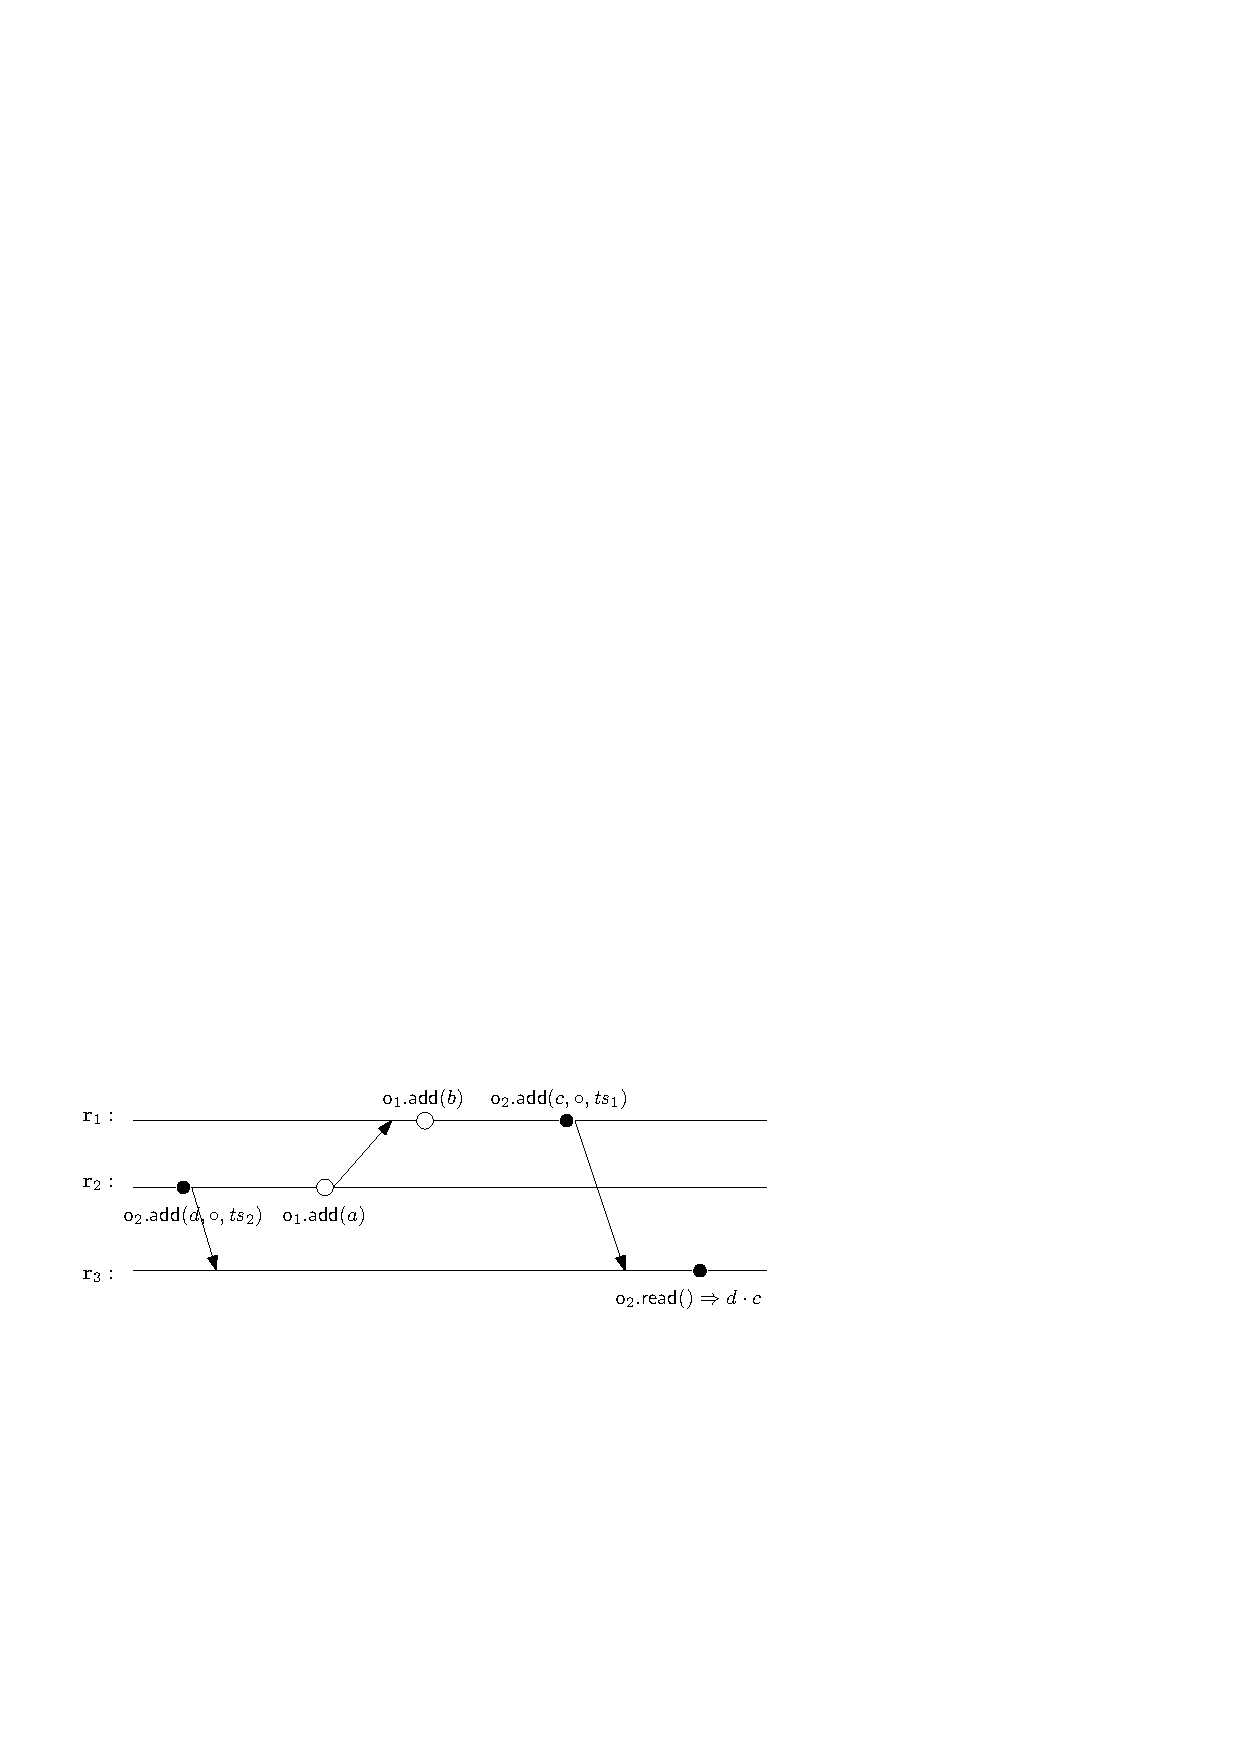
\includegraphics[width=0.6 \textwidth]{figures/MVReg-LWWReg-Nocd.pdf}
\vspace{-10pt}
  \caption{A failed example of composing a multi-value register with a last-write-win register (boxed operations), where $\mathit{ts}_1 < \mathit{ts}_2$.}
  \label{fig:a failed example of composing a multi-value register with a last-write-win register}
\end{figure}

The following lemma states that for a multi-object history, if its object use several t0-specifications and one t1-specification, and its visibility relation is transitive, then, $h$ is compositional. Its proof can be found in Appendix \ref{subsec:appendix proofs of lemma several t0-specifications and one t1-specification can be composed}.

\begin{restatable}{lemma}{composingTZeroAndOneTOne}
\label{lemma:several t0-specifications and one t1-specification can be composed}
Given a multi-object $h$, if its object use several t0-specifications and one t1-specification, and its visibility relation is transitive, then, $h$ is compositional.
\end{restatable}




\subsection{Composing Several t0-Specifications with Several T1-specification}
\label{lemma:composing several t0-specification with several t1-specification}

Composing several t0-specifications with several t1-specification does not hold in general. \figurename~\ref{fig:a failed example of composing two last-write-win registers} is a history $h$ that is a failed example of composing two last-write-win registers, where the operations of one LWW register are boxed, and the operations of the other LWW registers are not boxed. Here we assume that $\mathit{ts}_1 < \mathit{ts}_2 < \mathit{ts}_3$, and $\mathit{ts}'_1 < \mathit{ts}'_2$. Since LWW register is t1-specification, we can see that the projection of $h$ into operations of one LWW register is distributed linearization and the only possible linearization is $\mathit{write}(a,\mathit{ts}'_1) \cdot \mathit{write}(b,\mathit{ts}'_2)$, and the projection of $h$ into operations of the other LWW register is distributed linearization and the only possible linearization is $\mathit{write}(c,\mathit{ts}_1) \cdot \mathit{write}(d,\mathit{ts}_2) \cdot \mathit{write}(e,\mathit{ts}_3)$. However, $h$ is not distributed linearizable, since there is a a cycle.

\begin{figure}[t]
  \centering
  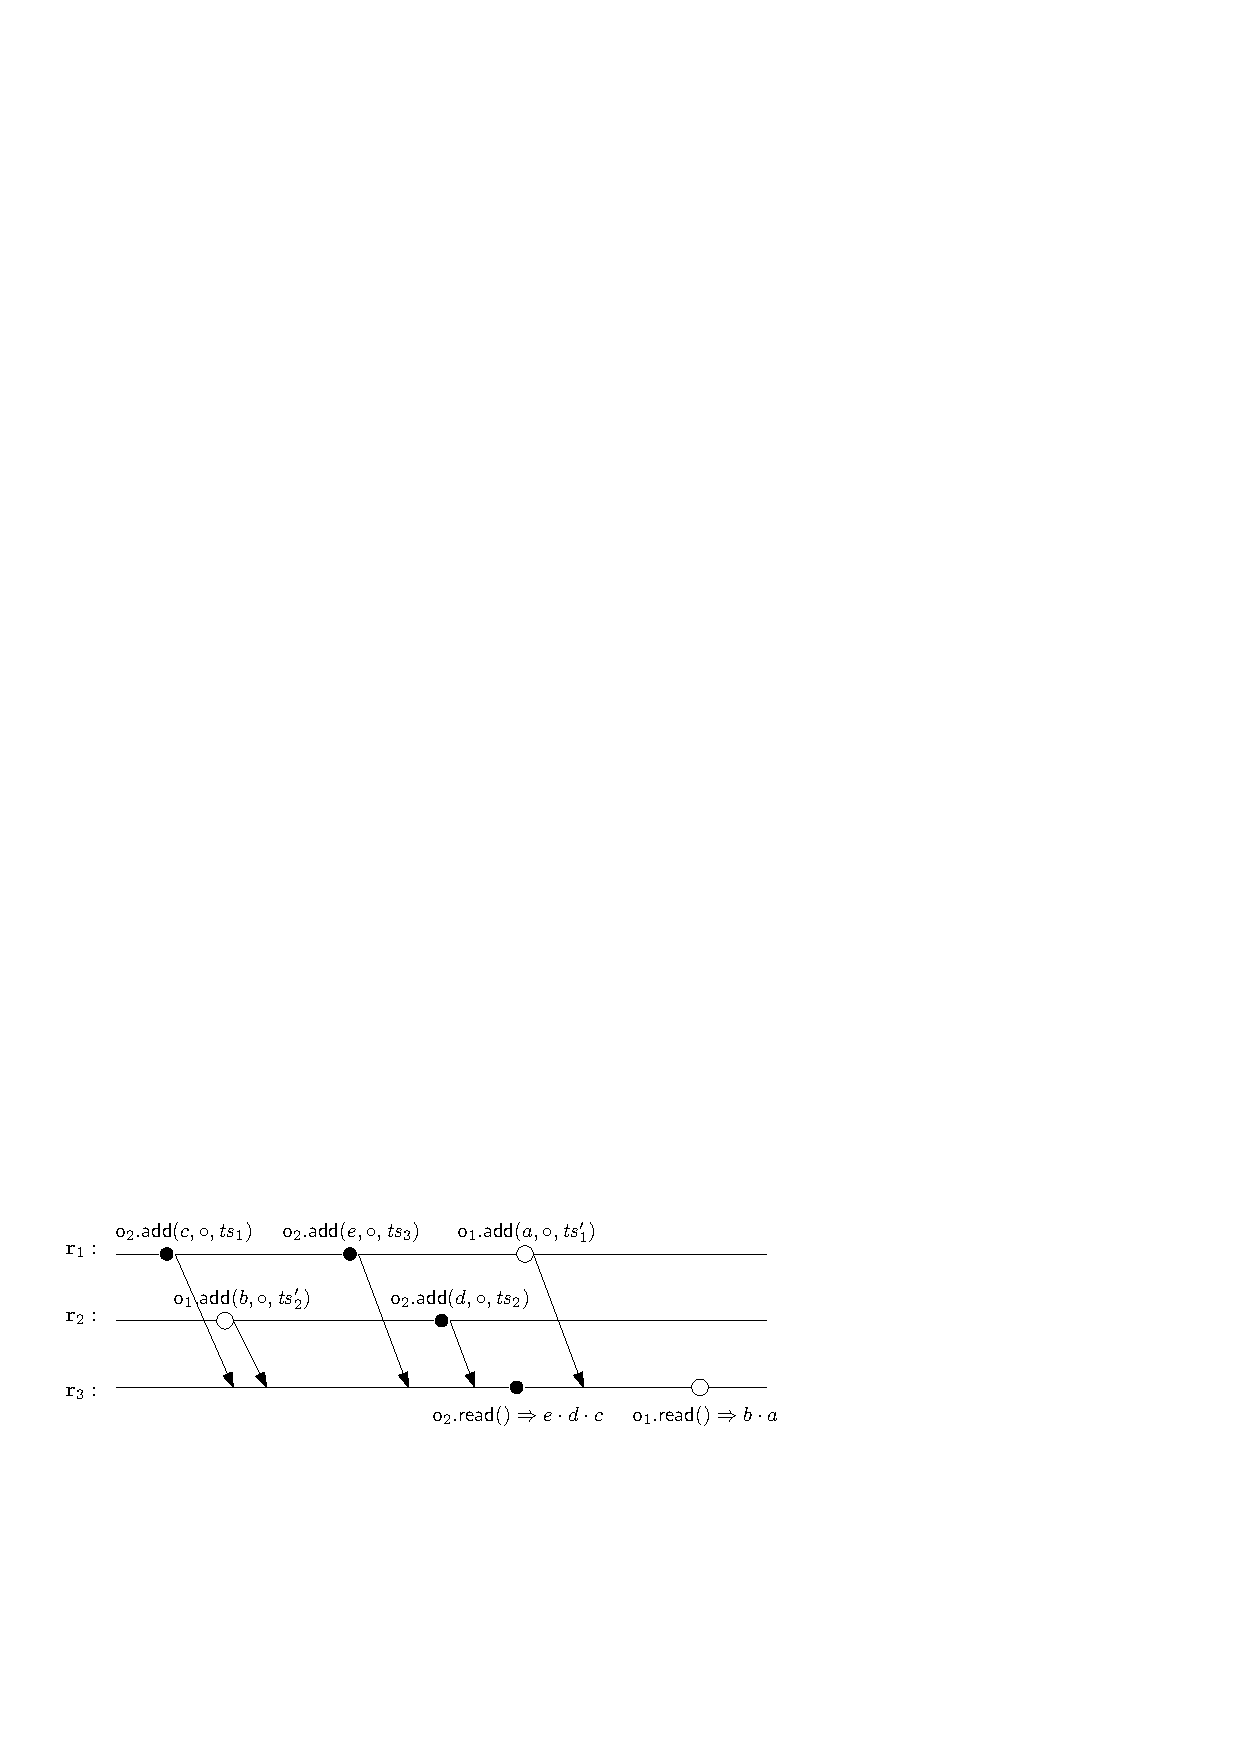
\includegraphics[width=0.7 \textwidth]{figures/LWWReg-LWWReg-NoSTS.pdf}
\vspace{-10pt}
  \caption{A failed example of composing two last-write-win registers (one object is boxed, the other is not), where $\mathit{ts}_1 < \mathit{ts}_2 < \mathit{ts}_3$, and $\mathit{ts}'_1 < \mathit{ts}'_2$.}
  \label{fig:a failed example of composing two last-write-win registers}
\end{figure}


A history $h$ satisfies causal-time-stamp, if: Given operation $o_1,\ldots,o_{\mathit{2k+2}}$ of $h$ that are of objects of t1-specification, if

\begin{itemize}
\setlength{\itemsep}{0.5pt}
\item[-] $(o_2,o_3)$ are of a same object, $\ldots$, $(o_{\mathit{2k}},o_{\mathit{2k+1}})$ are of a same object, $(o_{\mathit{2k+2}},o_1)$ are of a same object,

\item[-] $\mathit{ts}(o_2) < \mathit{ts}(o_2)$, $\ldots$, and $\mathit{ts}(o_{\mathit{2k}}) < \mathit{ts}(o_{\mathit{2k+1}})$,

\item[-] $(o_1,o_2), \ldots, (o_{\mathit{ek+1}},o_{\mathit{2k+2}}) \in \mathit{vis}$.
\end{itemize}

Then, we have $\mathit{ts}(o_1) < \mathit{ts}(o_{\mathit{2k+1}})$.

The following lemma states that for a multi-object history, if its object use several t0-specifications and several t1-specification, and it satisfies causal-time-stamp and its visibility relation is transitive, then, $h$ is compositional. Its proof can be found in Appendix \ref{subsec:appendix proofs of lemma several t0-specifications and several t1-specification can be composed}.

\begin{restatable}{lemma}{composingTZeroAndTOne}
\label{lemma:several t0-specifications and several t1-specification can be composed}
Given a multi-object $h$, if its object use several t0-specifications and several t1-specification, and it satisfies causal-time-stamp and its visibility relation is transitive, then, $h$ is compositional.
\end{restatable}






\subsection{Modified CRDT Implementation}
\label{subsec:modified CRDT implementation}

To ensure composing, we modify t1-algorithms as follows: The system supplies a method called $\mathit{updateGlobalTS}$, which supplies a time-stamp that is updated along the global system. When a method needs to generate new time-stamp, it calls this method to generate new time-stamp, and such process will also update the global time-stamp of this replica. When a method sends a message, the message should contain the current global time-stamp value. When a replica receives a message, it also use the global time-stamp value in message to update its own global time-stamp value. Moreover, the global time-stamp satisfies causal-time-stamp property.

The RGA algorithm after modification is as follows: Here a message contains the current global time-stamp value, and a replica update global time-stamp value is not explicitly written in code. Instead, such processes will be make explicit when constructing the operational semantics.

\begin{lstlisting}[caption={Pseudo-code of the Modified RGA}, captionpos=b,label={lst:modifier rga}]
  payload Ti-Tree N, Set Tomb
  initial N = @|$\emptyset$|@, Tomb = @|$\emptyset$|@

  addAfter(a,b) :
    atSource :
      precondition : b = @|$\circ$|@ or (b != @|$\circ$|@ and (b,_,_) @|$\in$|@ N and b @|$\not\in$|@ Tomb)
      let ts@|$_{\mathtt{a}}$|@ = updateGlobalTS()
      let ts@|$_{\mathtt{b}}$|@ = (b == @|$\circ$|@)?(0,r@|$_{0}$|@):(timestamp of b in N)
    downStream(a, ts@|$_{\mathtt{a}}$|@, ts@|$_{\mathtt{b}}$|@) :
      precondition: b = @|$\circ$|@ or (b != @|$\circ$|@ and (b, ts@|$_{\mathtt{b}}$|@,_) @|$\in$|@ N)
      N = N ts@|$\cup$|@ {(a, ts@|$_{\mathtt{a}}$|@, ts@|$_{\mathtt{b}}$|@)}

  remove(a) :
    atSource :
      precondition : a != @|$\emptyset$|@ and (a,_,_) @|$\in$|@ N and a @|$\notin$|@ Tomb
    downStream(a) :
      precondition : a != @|$\emptyset$|@ and (a,_,_) @|$\in$|@ N
      Tomb = Tomb @|$\cup$|@ {a}

  read() :
    return traverse(N, Tomb)
\end{lstlisting}


The following lemma states that the modified RGA is also t1-linearizable w.r.t $\mathit{list}_s^{\mathit{af}}$, and the modified LWW-register is t1-linearizable w.r.t $\mathit{reg}_s$. Its proof can be found in Appendix \ref{a}.

\begin{restatable}{lemma}{ModifiedRGAandLWWRegStillTOne}
\label{lemma:modified RGA and LWW-register is still t1-linearizable}
$\mathit{list}_s^{\mathit{af}}$ and $\mathit{reg}_s$ are t1-specifications.
\end{restatable}

Lamport's time-stamp is one way to implement global time-stamp, as stated by the following lemma. Its proof can be found in Appendix \ref{a}.

\begin{restatable}{lemma}{LamportTSasGlobalTS}
\label{lemma:lamport time-stamp as global time-stamp}
Lamport's time-stamp satisfies causal-time-stamp.
\end{restatable}








\subsection{Semantics of Multi Objects}
\label{subsec:semantics of multi objects}

When there is multiple objects, we say $(o_1,o_2) \in \mathit{vis}$, if either $(o_1,o_2) \in \mathit{ro}$, or $o_1$ is delivered to the replica of $o_2$ before $o_2$ happens. We consider CTDT implementation of t1-specifications use the time-stamp of Lamport's time-stamp: Each time-stamp is a tuple $(c,r)$ of a counter value $c \in \mathbb{N}$ and a replica identifier $r \in \mathbb{R}$; $(c_1,r_1) < (c_2,r_2)$, if $c_1 < c_2 \vee (c_1 = c_2 \wedge r_1 < r_2)$. To ensure compositionality of multiple objects, the following conditions needs to be satisfied:

\begin{itemize}
\setlength{\itemsep}{0.5pt}
\item[-] Cross-object-causal-delivery (COCD): We extend the notion of causal-delivery into multiple objects. Given two update operations $o_1$ and $o_2$, and assume $o_1$ is visible to $o_2$. Then, for each replica, once it receives $o_2$, it must be the case that $o_1$ has been previously received.

\item[-] Shared-time-stamp (STS): the objects of t1-specifications shares a counter $\mathit{sCtr}$. Each message carries a value of $\mathit{sCtr}$, and when generating new message, the value of $\mathit{sCtr}$ is also considered.
\end{itemize}



Based on shared-time-stamp,



Formally, given a set $\mathit{Objs}$ of objects, its semantics is defined as $\llbracket \mathit{Objs} \rrbracket_{\mathit{op}} = (\mathit{Config},\mathit{config}_0,\Sigma',\rightarrow)$ as in \figurename~\ref{fig:the semantics of multiple operation-based CRDT object}.


\begin{figure}[ht]
$\mathit{RState} = \mathit{Objs} \times \mathbb{R} \rightarrow \Sigma$

$\mathit{TState} = \mathbb{MID} \times \mathbb{MSG} \times \mathbb{R} \times \mathit{Objs}$

$\mathit{MsgHB} \subseteq \mathbb{MID} \times \mathbb{MID}$

$\mathit{MsgDel} \subseteq \mathbb{MID} \times \mathbb{R}$

$\mathit{Config} = \mathit{RState} \times \mathit{TState} \times \mathit{MsgHB} \times \mathit{MsgDel}$, $\mathit{config}_0 \in \mathit{Config}$.

$\Sigma' = \mathit{do}(\mathit{Objs} \times \mathbb{M} \times \mathbb{D} \times \mathbb{D} \times \mathbb{R} \times \mathbb{MID}) \cup \mathit{do}(\mathit{Objs} \times \mathbb{M} \times \mathbb{D} \times \mathbb{D} \times \mathbb{R}) \cup \mathit{receive}(\mathit{Objs} \times \mathbb{MID} \times \mathbb{R})$

\begin{itemize}
\setlength{\itemsep}{0.5pt}
\item[] $\begin{array}{l c}
   \bigfrac{
   \begin{array}{c}
     R(x,r) = \sigma, (x,r).\mathit{do}(\sigma,m,a) = (\sigma',b,\mathit{msg}), \mathit{msg} \neq \emptyset, \mathit{unique}(\mathit{mid}), \\
     S_1 = \{ (\mathit{mid}',\mathit{mid}) \vert (\mathit{mid'},r) \in \mathit{MsgDel} \}, S_2 = \{ (\mathit{mid}',\mathit{mid}) \vert \mathit{mid}' \in T, \mathit{mid}' \ is \ of \ replica \ r \}
   \end{array}}
     {(R,T,\mathit{msgHB},\mathit{MsgDel}) {\xrightarrow{\mathit{do}(x,m,a,b,r,\mathit{mid})}} (R[(x,r):\sigma'], T \cup \{ (\mathit{mid},\mathit{msg},r,x) \}, (\mathit{MsgHB} \cup S_1 \cup S_2)^*,\mathit{MsgDel})}
\end{array}$

\item[] $\begin{array}{l c}
   \bigfrac{
   \begin{array}{c}
     R(x,r) = \sigma, (x,r).\mathit{do}(\sigma,m,a) = (\sigma',b,\emptyset)
   \end{array}}
     {(R,T,\mathit{msgHB},\mathit{MsgDel}) {\xrightarrow{\mathit{do}(x,m,a,b,r)}} (R[(x,r):\sigma'], T \cup \{ (\mathit{mid},\mathit{msg},r) \}, \mathit{MsgHB},\mathit{MsgDel})}
\end{array}$

\item[-] $\begin{array}{l c}
   \bigfrac{
   \begin{array}{c}
      R(x,r) = \sigma, (x,r).\mathit{receive}(\sigma,\mathit{msg}) = \sigma', (\mathit{mid},\mathit{msg},r',x) \in T, r \neq r', \\
      (\mathit{mid},r) \notin \mathit{MsgDel}, \mathit{mid} \ is \ minimal \ w.r.t \ \mathit{MsgHB} \ among \ \{ \mathit{mid}' \vert (\mathit{mid}',r) \notin \mathit{MsgDel} \}
   \end{array}}
     {(R,T,\mathit{msgHB},\mathit{MsgDel}) {\xrightarrow{\mathit{receive}(x,\mathit{mid},r)}} (R,T,\mathit{MsgHB},\mathit{MsgDel} \cup \{ (\mathit{mid},r) \} )}
\end{array}$
\end{itemize}
\caption{The definition of semantics of $\llbracket \mathit{Objs} \rrbracket_{\mathit{op}}$}
\label{fig:the semantics of multiple operation-based CRDT object}
\end{figure}




$R$ is now a function from object and replica identifier to local state. Message and action also record its object. $\mathit{MsgHB}$ and $\mathit{MsgDel}$ now record the relation between messages of multiple objects. In each transition rule of \figurename~\ref{fig:the semantics of multiple operation-based CRDT object}, we deal with each object according to its CRDT implementations. Similarly, a sequence $l$ of actions is an execution of $\llbracket \mathit{Objs} \rrbracket_{\mathit{op}} = (\mathit{Config},\mathit{config}_0,\Sigma',\rightarrow)$, if there exists $(R,T,\mathit{MsgHB},\mathit{MsgDel}) \in \mathit{Config}$, such that $\mathit{config}_0 {\xrightarrow{ l }} (R,T,\mathit{MsgHB},\mathit{MsgDel})$. The semantics of $\mathit{Objs}$ is defined as the set of executions of $\llbracket \mathit{Objs} \rrbracket_{\mathit{op}}$.





A configuration $(R,T,\mathit{MsgHB},\mathit{MsgDel})$ is a snapshot of distributed system. $R$ gives the local state of each replica, and $T$ gives the set of messages that has been generated. Let $\mathbb{MID}$ be the set of message identifiers of message content. A message is a tuple $(\mathit{mid},\mathit{msg},r)$, where $\mathit{mid} \in \mathbb{MID}$ is the identifier, $\mathit{msg} \in \mathbb{MSG}$ is the message content, and $r$ is the original replica of message. $\mathit{MsgHB}$ is used to record the happen-before relation between messages: two messages $(\mathit{mid}_1,\mathit{mid}_2) \in \mathit{MsgHB}$ represents that the operation of $\mathit{mid}_1$ happens before the operation of $\mathit{mid}_2$. $\mathit{MsgDel}$ is used to record the message delivery relation between messages: $(\mathit{mid},r) \in \mathit{MsgDel}$ represents that message $\mathit{mid}_1$ has already been delivered to replica $r$. $\mathit{MsgHB}$ and $\mathit{MsgDel}$ are used to ensure message delivery requirements. $\mathit{config}_0$ is the initial configuration, which maps each replica into the initial local state, has no message, and with a empty happen-before relation and a empty message delivery relation.


Each element of $\Sigma'$ is called an action. $\rightarrow \in \mathit{Config} \times \Sigma' \times \mathit{Config}$ is the transition relation and describes a single step of distributed systems. The first rule in \figurename~\ref{fig:the semantics of a operation-based CRDT object} describes replica $r$ performs a update operation $m(a) \Rightarrow b$ and generates a message with message content $\mathit{msg}$. Here $\mathit{unique}$ is a function that ensures $\mathit{mid}$ be a fresh message identifier. We insert message identifier $\mathit{mid}$ into the happen-before relation and keeps the happen-before relation be transitive. The second rule describes replica $r$ performs a query operation $m(a) \Rightarrow b$ and thus does not generate message. Since no message is generated, the $\mathit{MsgHB}$ and $\mathit{MsgDel}$ tuples remain the same. The third rule describes delivery of a message to a replica $r$ other than its origin replica $r'$. By $(\mathit{mid},r) \notin \mathit{MsgDel}$, we ensure that $\mathit{mid}$ has not been previously delivered to replica $r$, and thus, each message be delivered to each replica at most once. By $\mathit{mid}$ being minimal w.r.t $\mathit{MsgHB}$ among $\{ \mathit{mid}' \vert (\mathit{mid}',r) \notin \mathit{MsgDel} \}$, we always choose a minimal element w.r.t $\mathit{MsgHB}$ among operations not been delivered to a replica, and thus, ensures causal-delivery.



\subsection{Proving in Multi-Objects Semantics}
\label{subsec:proving in multi-object semantics}


The formation of CRDT in this semantics is changed as follows,

The CRDT proved distributed linearizable are still distributed linearizable in this new semantics.
}
%%% Local Variables:
%%% mode: latex
%%% TeX-master: "draft"
%%% End:
